%%%%%%%%%%%%%%%%%%%%%%%%%%%%%%%%%%%%%%%%%%%%%%%%%%%%%%%%%%%%%%%%%%%%%%%%%%%%%%%%
%%%%%%%%%%%%%%%%%%%%%%%%%%%%%%%%%%%%%%%%%%%%%%%%%%%%%%%%%%%%%%%%%%%%%%%%%%%%%%%%
%%%%%%%%%%%%%%%%%%%%%%%%%%%%%%%%%%%%%%%%%%%%%%%%%%%%%%%%%%%%%%%%%%%%%%%%%%%%%%%%
%%%%%%%%%%%%%%%%%%%%%%%%%%%%%%%%%%%%%%%%%%%%%%%%%%%%%%%%%%%%%%%%%%%%%%%%%%%%%%%%
\chapter{Correction des systèmes asservis\label{chap-correc}}
%%%%%%%%%%%%%%%%%%%%%%%%%%%%%%%%%%%%%%%%%%%%%%%%%%%%%%%%%%%%%%%%%%%%%%%%%%%%%%%%
%%%%%%%%%%%%%%%%%%%%%%%%%%%%%%%%%%%%%%%%%%%%%%%%%%%%%%%%%%%%%%%%%%%%%%%%%%%%%%%%
%%%%%%%%%%%%%%%%%%%%%%%%%%%%%%%%%%%%%%%%%%%%%%%%%%%%%%%%%%%%%%%%%%%%%%%%%%%%%%%%
%%%%%%%%%%%%%%%%%%%%%%%%%%%%%%%%%%%%%%%%%%%%%%%%%%%%%%%%%%%%%%%%%%%%%%%%%%%%%%%%
\minitoc
\newpage
%%%%%%%%%%%%%%%%%%%%%%%%%%%%%%%%%%%%%%%%%%%%%%%%%%%%%%%%%%%%%%%%%%%%%%%%%%%%%%%%
%%%%%%%%%%%%%%%%%%%%%%%%%%%%%%%%%%%%%%%%%%%%%%%%%%%%%%%%%%%%%%%%%%%%%%%%%%%%%%%%
%%%%%%%%%%%%%%%%%%%%%%%%%%%%%%%%%%%%%%%%%%%%%%%%%%%%%%%%%%%%%%%%%%%%%%%%%%%%%%%%
\section{Nécessité de la correction}
%%%%%%%%%%%%%%%%%%%%%%%%%%%%%%%%%%%%%%%%%%%%%%%%%%%%%%%%%%%%%%%%%%%%%%%%%%%%%%%%
%%%%%%%%%%%%%%%%%%%%%%%%%%%%%%%%%%%%%%%%%%%%%%%%%%%%%%%%%%%%%%%%%%%%%%%%%%%%%%%%
%%%%%%%%%%%%%%%%%%%%%%%%%%%%%%%%%%%%%%%%%%%%%%%%%%%%%%%%%%%%%%%%%%%%%%%%%%%%%%%%
Nous avons établi et étudié en détail les différentes performances et 
exigences que l'on peut attendre de la réponse temporelle d'un système asservis.
Un système peut par exemple présenter des dépassements 
(\Cref{chap-model}), être précis, rapide (\Cref{chap-perf}), stable 
(\Cref{chap-stab}). Lorsque une réponse temporelle présente des performances
défaillantes par rapport à celles attendues par le cahier des charges (c.f 
la représentation schématique de la correction de 
la~\cref{fig-necessite_correction}), la notion de correction devient 
nécessaire. Une bonne correction est celle qui permet de respecter toutes
les exigences de l'ensemble des performances d'un cahier des charges donné. 
Par exemple, la figure ci-dessous présente un système asservis 
en boucle fermée avant et après correction. Il est clair que les performances
de rapidité et de précision ont été largement améliorées. Il est possible de 
constater également que le dépassement est largement réduit. Dans le cas, 
où un dépassement serait innaceptable, il faudrait alors imaginer une 
modification de la nature du système : un premier ordre ou un second ordre
en régime apériodique serait alors indispensable.

Le but de ce chapitre est de compiler une partie des résultats obtenue aux
chapitres précédents et de présenter la structure fonctionnelle de la 
correction. Nous nous intéresserons alors aux différents types de correcteurs 
élémentaires ainsi que de leurs compositions. Nous insisterons finalement
sur les correcteurs les plus utilisés que sont les correcteurs à avance de
phase, à retard de phase et les correcteurs PID.
L'exercice assez complet de ce chapitre permettra d'appliquer numériquement
en détail les principaux résultats du chapitre. 
\captionsetup{width=0.7\linewidth}
%-------------------------------------------------------------------------------
\begin{figure}[!b]
    \centering
    \tikzsetnextfilename{necessite_correction_chap_correction-ext}
    \pgfmathdeclarefunction{func}{1}{%
    \pgfmathparse{%
    1-((1./sqrt(1-#1*#1))*exp(-#1*x)*
    sin(deg(x)*sqrt(1-#1*#1)+atan(sqrt(1-#1*#1)/#1)))
    }%
}

\begin{tikzpicture}
    \begin{axis}
    [   legend style={draw=none},
        legend pos=outer north east,
        legend cell align={left},
        width=0.6\textwidth,
        axis line style = thick,
        xmin=0,
        xmax=30,
        ymin=0,
        ymax=1.75,
        xlabel={$t$},
        ylabel={$s(t)$},
        xtick={},
        xticklabels={},
        ytick={1.15},
        yticklabels={$E_0$},
        label style={font=\Large},
        clip=false
    ]
    \addplot[signalr,domain=0:30] {func(0.15)};
    \addlegendentry{Non Corrigé}
    \addplot[signalg,domain=0:30] {1.15*func(0.707)};
    \addlegendentry{Corrigé}
    \addplot[signaln,domain=0:30] {1.15}      ;
    \addplot[signalr,dashed,domain=0:30,draw opacity=0.5] {1.0};
    \draw[latex-latex, col4, line width=1.0pt] (axis cs:31,1)  -- 
        node[midway,xshift=1.3cm, text width=2cm, align=center] 
        {\textbf{\'Ecart \\(Précision)}} 
        (axis cs:31,1.15) ;
    \draw[-latex, col4, line width=2.0pt]      (axis cs:3.2,1) -- 
        node[midway,xshift=1.6cm,yshift=0.8cm] {\textbf{Dépassement}}
        (axis cs:3.2,1.63) ;
    \draw[col4, line width=1.0pt] (axis cs:19.5,0)  -- 
        node[yshift=-2.7cm,text width=2cm,align=center] 
        {\textbf{$\boldsymbol{t_{5\%}}$\\(Rapidité)}} 
        (axis cs:19.5,0.95) ;
    \end{axis}
\end{tikzpicture}

    \caption{Représentation schématique de la correction de la réponse 
             temporelle d'un système asservi. (en rouge) Le système non corrigé, 
             présente un important dépassement, il est lent et peu précis. 
             (en vert) Le système corrigé présente de meilleurs performances 
             pour tous les critères précédents.\label{fig-necessite_correction}}
\end{figure}
%-------------------------------------------------------------------------------
\captionsetup{width=0.9\linewidth}
\clearpage
%%%%%%%%%%%%%%%%%%%%%%%%%%%%%%%%%%%%%%%%%%%%%%%%%%%%%%%%%%%%%%%%%%%%%%%%%%%%%%%%
%%%%%%%%%%%%%%%%%%%%%%%%%%%%%%%%%%%%%%%%%%%%%%%%%%%%%%%%%%%%%%%%%%%%%%%%%%%%%%%%
%%%%%%%%%%%%%%%%%%%%%%%%%%%%%%%%%%%%%%%%%%%%%%%%%%%%%%%%%%%%%%%%%%%%%%%%%%%%%%%%
\section{Structure de la correction}
%%%%%%%%%%%%%%%%%%%%%%%%%%%%%%%%%%%%%%%%%%%%%%%%%%%%%%%%%%%%%%%%%%%%%%%%%%%%%%%%
%%%%%%%%%%%%%%%%%%%%%%%%%%%%%%%%%%%%%%%%%%%%%%%%%%%%%%%%%%%%%%%%%%%%%%%%%%%%%%%%
%%%%%%%%%%%%%%%%%%%%%%%%%%%%%%%%%%%%%%%%%%%%%%%%%%%%%%%%%%%%%%%%%%%%%%%%%%%%%%%%
Comme nous avons pu l'observer au cours de chapitres précédents, les 
performances d'un système asservis dépendent essentiellement de la fonction
de transfert en boucle ouverte. Corriger un système revient à modifier 
cette~\gls{ftbo} pour obtenir les performances souhaitées. Il existe un grand
nombre de structure de la correction, nous souhaitons tout d'abord les 
présenter avant de faire une étude plus détaillé de la structure la plus 
classiquement rencontrée. 

Notons tout abord que la correction ou un correcteur est une fonction 
de transfert qui \textbf{élabore une commande $u(t)$ à partir d'un écart 
$\epsilon(t)$}. Nous noterons un correcteur par la fonction de transfert
$C(p)$ et sa représentation en schéma-bloc comme ci-dessous.
%-------------------------------------------------------------------------------
\begin{center}
    \tikzsetnextfilename{bs_correction_chap_correction-ext}
    \begin{tikzpicture}
    \bs[$\epsilon(p)$][$C(p)$][Correcteur][$U(p)$]
\end{tikzpicture}

\end{center}
%-------------------------------------------------------------------------------
Cependant, il existe différentes façon de placer un correcteur dans un 
asservissement. Si il est vraie qu'un asservissement présente toujours une
boucle de contre-réaction, \textbf{la correction peut se faire soit en série, 
soit en réaction ou soit dans une structure mixte (appelée série-réaction)}.
À noter, que c'est la correction en série qui est la plus fréquemment rencontrée
et c'est celle-ci que nous étudierons en détail dans ce chapitre.
%%%%%%%%%%%%%%%%%%%%%%%%%%%%%%%%%%%%%%%%%%%%%%%%%%%%%%%%%%%%%%%%%%%%%%%%%%%%%%%%
\paragraph{Correction en série}
%%%%%%%%%%%%%%%%%%%%%%%%%%%%%%%%%%%%%%%%%%%%%%%%%%%%%%%%%%%%%%%%%%%%%%%%%%%%%%%%
Dans une correction en série, le correcteur $C(p)$ est placé dans la chaîne
directe de l'asservissement. Il élabore une commande $U(p)$ pour le système en 
boucle ouverte non corrigée $H(p)$. Le schéma-bloc
d'une telle correction est représentée ci-dessous:
%-------------------------------------------------------------------------------
\begin{center}
    \tikzsetnextfilename{correction_serie_chap_correction-ext}
    \begin{tikzpicture}
    \corrbruni
\end{tikzpicture}

\end{center}
%-------------------------------------------------------------------------------
En appliquant l'algèbre de bloc, il est assez simple de déterminer la forme de
la commande pour ce type de correction :
\[
    U(p)=C(p)\epsilon(p)
\]
À partir de la fonction de transfert en boucle ouverte du système corrigé 
$H_{BO}$, telle que :
\[
    H_{BO}(p)=C(p)H(p),
\]
la fonction de transfert en boucle fermée est simplement donnée par :
\[
    H_{BF}(p)=\dfrac{C(p)H(p)}{1+C(p)H(p)}.
\]
%%%%%%%%%%%%%%%%%%%%%%%%%%%%%%%%%%%%%%%%%%%%%%%%%%%%%%%%%%%%%%%%%%%%%%%%%%%%%%%%
\paragraph{Correction en réaction}
%%%%%%%%%%%%%%%%%%%%%%%%%%%%%%%%%%%%%%%%%%%%%%%%%%%%%%%%%%%%%%%%%%%%%%%%%%%%%%%%
Dans le cas d'une correction en réaction, la commande $U(p)$ est élaborée 
à partir de l'écart $\epsilon(p)$ et de l'image de la sortie par le correcteur
$C(p)S(p)$, cette relation s'écrit simplement : 
\[
    U(p)=\epsilon(p)-C(p)S(p)
\]
Le schéma-bloc de cette correction est donnée ci-dessous :
%-------------------------------------------------------------------------------
\begin{center}
    \tikzsetnextfilename{correction_reaction_chap_correction-ext}
    \begin{tikzpicture}
    \sbEntree{E1}
    \sbComp[4.5]{comp}{E1}
    \sbRelier[$E(p)$]{E1}{comp}
    \sbComp[4.5]{comp2}{comp}
    \sbRelier[$\epsilon(p)$]{comp}{comp2}
    \sbBloc[3]{B1}{$H(p)$}{comp2}
    \sbRelier[$U(p)$]{comp2}{B1}
    \sbSortie[6]{S1}{B1}
    \sbRelier{B1}{S1}
    \sbNomLien[0.8]{S1}{$S(p)$}
    \sbRenvoi[8]{B1-S1}{comp}{}
    \sbDecaleNoeudy{B1}{R}
    \sbBlocr[-1.75]{R1}{$C(p)$}{R}
    \sbRelieryx{B1-S1}{R1}
    \sbRelierxy{R1}{comp2}
\end{tikzpicture}

\end{center}
%-------------------------------------------------------------------------------
Attention, le correcteur ne se trouve pas dans la
chaîne de retour (ce qui aurait un effet très peu différent de la 
correction en série puisque la fonction de transfert en boucle ouverte serait
alors la même)  

En appliquant une nouvelle fois l'algèbre de bloc à cette correction, on
obtient les relations suivantes pour les fonctions de transfert en boucle 
ouverte et boucle fermée
\[
    H_{BO}(p)=\dfrac{H(p)}{1+C(p)H(p)}
\]
\[
    H_{BF}(p)=\dfrac{H(p)}{1+H(p)+C(p)H(p)}
\]
Comme on peut l'observer, dans une telle correction la~\gls{ftbo} est de la
forme d'un asservissement. On peut dire de façon imagée que l'on corrige par
un asservissement interne.
%%%%%%%%%%%%%%%%%%%%%%%%%%%%%%%%%%%%%%%%%%%%%%%%%%%%%%%%%%%%%%%%%%%%%%%%%%%%%%%%
\paragraph{Correction en série-réaction}
%%%%%%%%%%%%%%%%%%%%%%%%%%%%%%%%%%%%%%%%%%%%%%%%%%%%%%%%%%%%%%%%%%%%%%%%%%%%%%%%
Dans le cas d'une correction en série-réaction, on combine les deux structures
précédentes (série et réaction) en une seul correction. Dans ce cas, deux
correcteurs $C_1(p)$ et $C_2(p)$ sont nécessaires respectivement 
en correction en série et réaction.
%-------------------------------------------------------------------------------
\begin{center}
    \tikzsetnextfilename{correction_serie-reaction_chap_correction-ext}
    \input{tikz/correction_serie-reaction_chap_correction.tex}
\end{center}
%-------------------------------------------------------------------------------
%\[
%    U(p)=C_1(p)\epsilon(p)-C_2(p)S(p)
%\]
%\[
%    H_{BO}(p)=\dfrac{C_1(p)H(p)}{1+C_2(p)H(p)}
%\]
%\[
%    H_{BF}(p)=\dfrac{C_1(p)H(p)}{1+C_1(p)H(p)+C_2(p)H(p)}
%\]
Nous envisagerons que la correction en série par la suite.
%%%%%%%%%%%%%%%%%%%%%%%%%%%%%%%%%%%%%%%%%%%%%%%%%%%%%%%%%%%%%%%%%%%%%%%%%%%%%%%%
%%%%%%%%%%%%%%%%%%%%%%%%%%%%%%%%%%%%%%%%%%%%%%%%%%%%%%%%%%%%%%%%%%%%%%%%%%%%%%%%
%%%%%%%%%%%%%%%%%%%%%%%%%%%%%%%%%%%%%%%%%%%%%%%%%%%%%%%%%%%%%%%%%%%%%%%%%%%%%%%%
\section{Correcteurs élémentaires P, I et D}
%%%%%%%%%%%%%%%%%%%%%%%%%%%%%%%%%%%%%%%%%%%%%%%%%%%%%%%%%%%%%%%%%%%%%%%%%%%%%%%%
%%%%%%%%%%%%%%%%%%%%%%%%%%%%%%%%%%%%%%%%%%%%%%%%%%%%%%%%%%%%%%%%%%%%%%%%%%%%%%%%
%%%%%%%%%%%%%%%%%%%%%%%%%%%%%%%%%%%%%%%%%%%%%%%%%%%%%%%%%%%%%%%%%%%%%%%%%%%%%%%%
%%%%%%%%%%%%%%%%%%%%%%%%%%%%%%%%%%%%%%%%%%%%%%%%%%%%%%%%%%%%%%%%%%%%%%%%%%%%%%%%
%%%%%%%%%%%%%%%%%%%%%%%%%%%%%%%%%%%%%%%%%%%%%%%%%%%%%%%%%%%%%%%%%%%%%%%%%%%%%%%%
\subsection{Correcteur P}
%%%%%%%%%%%%%%%%%%%%%%%%%%%%%%%%%%%%%%%%%%%%%%%%%%%%%%%%%%%%%%%%%%%%%%%%%%%%%%%%
%%%%%%%%%%%%%%%%%%%%%%%%%%%%%%%%%%%%%%%%%%%%%%%%%%%%%%%%%%%%%%%%%%%%%%%%%%%%%%%%
\index{Correcteur!Proportionnel (P)}
%-------------------------------------------------------------------------------
\begin{center}
    \tikzsetnextfilename{p_chap_correction-ext}
    \begin{tikzpicture}
    \sbStyleBloc{col4}
    \bs[$\epsilon(p)$][$k_p$][][$U(p)$]
\end{tikzpicture}

\end{center}
%-------------------------------------------------------------------------------
%-------------------------------------------------------------------------------
\begin{bequation}[ams align]
    C_{\text{P}}(p)=k_p 
\end{bequation}
%-------------------------------------------------------------------------------
%%%%%%%%%%%%%%%%%%%%%%%%%%%%%%%%%%%%%%%%%%%%%%%%%%%%%%%%%%%%%%%%%%%%%%%%%%%%%%%%
%%%%%%%%%%%%%%%%%%%%%%%%%%%%%%%%%%%%%%%%%%%%%%%%%%%%%%%%%%%%%%%%%%%%%%%%%%%%%%%%
\subsection{Correcteur I}
%%%%%%%%%%%%%%%%%%%%%%%%%%%%%%%%%%%%%%%%%%%%%%%%%%%%%%%%%%%%%%%%%%%%%%%%%%%%%%%%
%%%%%%%%%%%%%%%%%%%%%%%%%%%%%%%%%%%%%%%%%%%%%%%%%%%%%%%%%%%%%%%%%%%%%%%%%%%%%%%%
\index{Correcteur!Intégral (I)}
%-------------------------------------------------------------------------------
\begin{center}
    \tikzsetnextfilename{i_chap_correction-ext}
    \begin{tikzpicture}
    \sbStyleBloc{col3}
    \bs[$\epsilon(p)$][$\dfrac{1}{\tau_i p}$][][$U(p)$]
\end{tikzpicture}

\end{center}
%-------------------------------------------------------------------------------
%-------------------------------------------------------------------------------
\begin{bequation}[ams align]
    C_{\text{I}}(p)=\dfrac{1}{\tau_i p} 
\end{bequation}
%-------------------------------------------------------------------------------
%%%%%%%%%%%%%%%%%%%%%%%%%%%%%%%%%%%%%%%%%%%%%%%%%%%%%%%%%%%%%%%%%%%%%%%%%%%%%%%%
%%%%%%%%%%%%%%%%%%%%%%%%%%%%%%%%%%%%%%%%%%%%%%%%%%%%%%%%%%%%%%%%%%%%%%%%%%%%%%%%
\subsection{Correcteur D}
%%%%%%%%%%%%%%%%%%%%%%%%%%%%%%%%%%%%%%%%%%%%%%%%%%%%%%%%%%%%%%%%%%%%%%%%%%%%%%%%
%%%%%%%%%%%%%%%%%%%%%%%%%%%%%%%%%%%%%%%%%%%%%%%%%%%%%%%%%%%%%%%%%%%%%%%%%%%%%%%%
\index{Correcteur!Dérivé (D)}
%-------------------------------------------------------------------------------
\begin{center}
    \tikzsetnextfilename{d_chap_correction-ext}
    \begin{tikzpicture}
    \sbStyleBloc{col1}
    \bs[$\epsilon(p)$][$\tau_d p$][][$U(p)$]
\end{tikzpicture}

\end{center}
%-------------------------------------------------------------------------------
%-------------------------------------------------------------------------------
\begin{bequation}[ams align]
    C_{\text{D}}^{\text{idéal}}(p)=\tau_d p 
\end{bequation}
%-------------------------------------------------------------------------------
Le correcteur dérivé sous cette forme est purement théorique, notamment parce
que le gain est infini lorsque la pulsation tend vers l'infini.

Une solution technologique permet de réaliser une forme approché :
\[
    C_{\text{D}}^{\text{réel}}(p)=\dfrac{\tau_d p}{1+\tau p}
\]
en choissisant un temps $\tau\ll\tau_d$, cette fonction de transfert se comporte
comme un correcteur dérivé idéal. On parle également dans ce cas de correcteur
\og D filtré\fg.
%%%%%%%%%%%%%%%%%%%%%%%%%%%%%%%%%%%%%%%%%%%%%%%%%%%%%%%%%%%%%%%%%%%%%%%%%%%%%%%%
%%%%%%%%%%%%%%%%%%%%%%%%%%%%%%%%%%%%%%%%%%%%%%%%%%%%%%%%%%%%%%%%%%%%%%%%%%%%%%%%
%%%%%%%%%%%%%%%%%%%%%%%%%%%%%%%%%%%%%%%%%%%%%%%%%%%%%%%%%%%%%%%%%%%%%%%%%%%%%%%%
\section{Correcteurs composés}
%%%%%%%%%%%%%%%%%%%%%%%%%%%%%%%%%%%%%%%%%%%%%%%%%%%%%%%%%%%%%%%%%%%%%%%%%%%%%%%%
%%%%%%%%%%%%%%%%%%%%%%%%%%%%%%%%%%%%%%%%%%%%%%%%%%%%%%%%%%%%%%%%%%%%%%%%%%%%%%%%
%%%%%%%%%%%%%%%%%%%%%%%%%%%%%%%%%%%%%%%%%%%%%%%%%%%%%%%%%%%%%%%%%%%%%%%%%%%%%%%%
Comme leurs noms l'indique, les correcteurs composés combinent plusieurs
des correcteurs élémentaires présentés précedemment.
%%%%%%%%%%%%%%%%%%%%%%%%%%%%%%%%%%%%%%%%%%%%%%%%%%%%%%%%%%%%%%%%%%%%%%%%%%%%%%%%
%%%%%%%%%%%%%%%%%%%%%%%%%%%%%%%%%%%%%%%%%%%%%%%%%%%%%%%%%%%%%%%%%%%%%%%%%%%%%%%%
\subsection{Correcteur PI}
%%%%%%%%%%%%%%%%%%%%%%%%%%%%%%%%%%%%%%%%%%%%%%%%%%%%%%%%%%%%%%%%%%%%%%%%%%%%%%%%
%%%%%%%%%%%%%%%%%%%%%%%%%%%%%%%%%%%%%%%%%%%%%%%%%%%%%%%%%%%%%%%%%%%%%%%%%%%%%%%%
\index{Correcteur!Proportionnel Intégral (PI)}
%-------------------------------------------------------------------------------
\begin{figure}
    \centering
    \tikzsetnextfilename{bode_pi_gain_chap_correction-ext}
    \input{tikz/bode_pi_gain_chap_correction.tex}
    
    \tikzsetnextfilename{bode_pi_phase_chap_correction-ext}
    \input{tikz/bode_pi_phase_chap_correction.tex}
    \caption{Diagramme de Bode du correcteur à effet proportionnel et intégral.}
\end{figure}
%-------------------------------------------------------------------------------
%-------------------------------------------------------------------------------
\begin{center}
    \tikzsetnextfilename{pi_chap_correction-ext}
     \begin{tikzpicture}
    \sbEntree{E1}
    \sbStyleBloc{col4}
    \sbBloc[3]{B1}{$k_p$}{E1}
    \sbRelier[$\epsilon(p)$]{E1}{B1}
    \sbStyleBloc{col3}
    \sbBloc[3]{B2}{$\dfrac{1}{\tau_i p}$}{B1}
    \sbRelier{B1}{B2}
    \sbCompSum[5]{C1}{B2}{+}{}{+}{ }
    \sbRelier{B2}{C1}
    \sbStyleBloc{col1}
    \sbSortie[3]{S1}{C1}
    \sbRelier[$U(p)$]{C1}{S1}
    \sbRenvoi[-4]{B1-B2}{C1}{}
    \node at ($(B1)+(0.88,0.7)$) {\textcolor{col4}{P}};
    \node at ($(B2)+(0.88,0.7)$) {\textcolor{col3}{I}};
\end{tikzpicture}

\end{center}
%-------------------------------------------------------------------------------
\[
    U(p)=k_p\left(1+\dfrac{1}{\tau_i p}\right)\epsilon(p)
\]
%-------------------------------------------------------------------------------
\begin{bequation}[ams align]
    C_{\text{PI}}=k_p\left(\dfrac{1+\tau_i p}{\tau_i p}\right)
\end{bequation}
%-------------------------------------------------------------------------------
%%%%%%%%%%%%%%%%%%%%%%%%%%%%%%%%%%%%%%%%%%%%%%%%%%%%%%%%%%%%%%%%%%%%%%%%%%%%%%%%
%%%%%%%%%%%%%%%%%%%%%%%%%%%%%%%%%%%%%%%%%%%%%%%%%%%%%%%%%%%%%%%%%%%%%%%%%%%%%%%%
\subsection{Correcteur PD}
%%%%%%%%%%%%%%%%%%%%%%%%%%%%%%%%%%%%%%%%%%%%%%%%%%%%%%%%%%%%%%%%%%%%%%%%%%%%%%%%
%%%%%%%%%%%%%%%%%%%%%%%%%%%%%%%%%%%%%%%%%%%%%%%%%%%%%%%%%%%%%%%%%%%%%%%%%%%%%%%%
\index{Correcteur!Proportionnel Dérivé (PD)}
%-------------------------------------------------------------------------------
\begin{figure}
    \centering
    \tikzsetnextfilename{bode_pd_gain_chap_correction-ext}
    \begin{tikzpicture}[trim axis left]
    \begin{axis}[
    ticklabel style = {font=\footnotesize},
    width=0.9\textwidth,
    height=0.25\textheight,
    ylabel={Gain (\si{\decibel})},
    xtick={1e-4,1e-3,1e-2,1e-1,1,1e1,1e2,1e3,1e4,1e5},
    ytick={0,10,20,30,40},
    xticklabels={$10^{-4}$,$10^{-3}$,$10^{-2}$,$10^{-1}$,
                 $10^{0}$,$10^{1}$,$10^{2}$,$10^{3}$,$10^{4}$,$10^{5}$},
    yticklabels={0,10,20,30,40},
    xmode=log,ymode=normal,
    xmin=1e-2, xmax=1e2,
    ymin=0, ymax=30,
    grid=both,
    major grid style={black!40},
]
    \pgfmathsetmacro{\td}{1.000001} 
    \pgfmathsetmacro{\wtd}{(1/\td)} 
    \pgfmathsetmacro{\tau}{0.1} 
    \pgfmathsetmacro{\wt}{1.0/\tau} 
    \addplot[ultra thick, col3,domain=1e-2:1e2, samples=201]    
            {10*log10(1+\td*\td*x*x)-10*log10(1+\tau*\tau*x*x)};
    \addplot[ultra thick,col1,domain=1e-2:1e2, samples=201]    
            {10*log10(1+\td*\td*x*x)};
    \addplot[line width=2pt,col4,dashed,domain=\wtd:1e2, samples=51] 
            {20*log10(x)};
    \addplot[line width=2pt,col4,dashed,domain=1e-2:\wtd, samples=51] {0};
\end{axis}
\end{tikzpicture}

    
    \tikzsetnextfilename{bode_pd_phase_chap_correction-ext}
    \begin{tikzpicture}[trim axis left]
\begin{axis}[
    ticklabel style = {font=\footnotesize},
    width=0.9\textwidth,
    height=0.25\textheight,
    xlabel={Pulsation (\si{\radian\per\second})},
    ylabel={Phase (\degreeSI)},
    xtick={1e-4,1e-3,1e-2,1e-1,1,1e1,1e2,1e3,1e4,1e5},
    ytick={0,15,30,45,60,75,90},
    yticklabels={0,,30,,60,,90},
    xticklabels={$10^{-4}$,$10^{-3}$,$10^{-2}$,$10^{-1}$,$10^{0}$,
                 $10^{1}$,$10^{2}$,$10^{3}$,$10^{4}$,$10^{5}$},
    xmode=log,ymode=normal,
    xmin=1e-2, xmax=1e2,
    ymin=0, ymax=90,
    grid=both,
    major grid style={black!40},
    %clip=false
]
    \pgfmathsetmacro{\td}{1.0} 
    \pgfmathsetmacro{\wtd}{1.0/\td} 
    \pgfmathsetmacro{\tau}{0.1} 
    \pgfmathsetmacro{\wt}{1.0/\tau} 
    \addplot[ultra thick, col1,domain=1e-2:1e2, samples=201] 
    {atan2(\td*x,1)};
    \addplot[ultra thick, col3,domain=1e-2:1e2, samples=201] 
    {atan2(\td*x,1)-atan2(\tau*x,1)};
    \addplot[line width=2pt,col4,dashed,domain=1e-2:\wtd, samples=51] {0};
    \addplot[line width=2pt,col4,dashed,domain=\wtd:1e2, samples=51] {90};
    \draw[line width=2pt,col4,dashed] 
         (axis cs:\wtd,0) -- (axis cs:\wtd,90);
\end{axis}
\end{tikzpicture}

    \caption{Diagramme de Bode du correcteur à effet proportionnel et dérivé.}
\end{figure}
%-------------------------------------------------------------------------------
%-------------------------------------------------------------------------------
\begin{center}
    \tikzsetnextfilename{pd_chap_correction-ext}
    \begin{tikzpicture}
    \sbEntree{E1}
    \sbStyleBloc{col4}
    \sbBloc[3]{B1}{$k_p$}{E1}
    \sbRelier[$\epsilon(p)$]{E1}{B1}
    \sbStyleBloc{col1}
    \sbBloc[3]{B3}{$\tau_d p$}{B1}
    \sbRelier{B1}{B3}
    \sbCompSum[5]{C2}{B3}{+}{}{+}{ }
    \sbRelier{B3}{C2}
    \sbSortie[3]{S1}{C2}
    \sbRelier[$U(p)$]{C2}{S1}
    \sbRelier{C2}{S1}
    \sbRenvoi[-4]{B1-B3}{C2}{}
    \node at ($(B1)+(0.88,0.7)$) {\textcolor{col4}{P}};
    \node at ($(B3)+(0.88,0.7)$) {\textcolor{col1}{D}};
\end{tikzpicture}

\end{center}
%-------------------------------------------------------------------------------
\[
    U(p)=k_p\left(1+\dfrac{1}{\tau_i p}\right)\epsilon(p)
\]
%-------------------------------------------------------------------------------
\begin{bequation}[ams align]
    C_{\text{PD}}=k_p\left(1+\tau_d p\right)
\end{bequation}
%-------------------------------------------------------------------------------
À l'instar du correcteur dérivé élémentaire, le correcteur composé PD présente
une forme approché/filtré :
\[
    C_{\text{PD}}=k_p\dfrac{1+\tau_d p}{1+\tau p}
\]
avec $\tau\ll\tau_d$
%%%%%%%%%%%%%%%%%%%%%%%%%%%%%%%%%%%%%%%%%%%%%%%%%%%%%%%%%%%%%%%%%%%%%%%%%%%%%%%%
%%%%%%%%%%%%%%%%%%%%%%%%%%%%%%%%%%%%%%%%%%%%%%%%%%%%%%%%%%%%%%%%%%%%%%%%%%%%%%%%
%%%%%%%%%%%%%%%%%%%%%%%%%%%%%%%%%%%%%%%%%%%%%%%%%%%%%%%%%%%%%%%%%%%%%%%%%%%%%%%%
\section{Correcteurs à avance et retard de phase}
%%%%%%%%%%%%%%%%%%%%%%%%%%%%%%%%%%%%%%%%%%%%%%%%%%%%%%%%%%%%%%%%%%%%%%%%%%%%%%%%
%%%%%%%%%%%%%%%%%%%%%%%%%%%%%%%%%%%%%%%%%%%%%%%%%%%%%%%%%%%%%%%%%%%%%%%%%%%%%%%%
%%%%%%%%%%%%%%%%%%%%%%%%%%%%%%%%%%%%%%%%%%%%%%%%%%%%%%%%%%%%%%%%%%%%%%%%%%%%%%%%
%%%%%%%%%%%%%%%%%%%%%%%%%%%%%%%%%%%%%%%%%%%%%%%%%%%%%%%%%%%%%%%%%%%%%%%%%%%%%%%%
%%%%%%%%%%%%%%%%%%%%%%%%%%%%%%%%%%%%%%%%%%%%%%%%%%%%%%%%%%%%%%%%%%%%%%%%%%%%%%%%
\subsection{Correcteur à avance de phase}
%%%%%%%%%%%%%%%%%%%%%%%%%%%%%%%%%%%%%%%%%%%%%%%%%%%%%%%%%%%%%%%%%%%%%%%%%%%%%%%%
%%%%%%%%%%%%%%%%%%%%%%%%%%%%%%%%%%%%%%%%%%%%%%%%%%%%%%%%%%%%%%%%%%%%%%%%%%%%%%%%
\index{Correcteur!à avance de phase (AP)}
Le correcteur à avance de phase (AP) est défini par la fonction de transfert :
%-------------------------------------------------------------------------------
\begin{bequation}[ams align]
    C_{\text{AP}}(p)=k_p\dfrac{1+\alpha\tau p}{1+\tau p} 
\end{bequation}
%-------------------------------------------------------------------------------
avec $\alpha>1$.
%-------------------------------------------------------------------------------
\begin{figure}
    \centering
    \tikzsetnextfilename{bode_avancedephase_gain_chap_correction-ext}
    \begin{tikzpicture}[trim axis left]
    \begin{axis}[
    ticklabel style = {font=\footnotesize},
    width=0.9\textwidth,
    height=0.25\textheight,
    ylabel={Gain (\si{\decibel})},
    xtick={1e-4,1e-3,1e-2,1e-1,1,1e1,1e2,1e3,1e4,1e5},
    ytick={0,1,2,3,4,5,6,7,8,9,10,11,12,13,14,15},
    xticklabels={$10^{-4}$,$10^{-3}$,$10^{-2}$,$10^{-1}$,
                 $10^{0}$,$10^{1}$,$10^{2}$,$10^{3}$,$10^{4}$,$10^{5}$},
    yticklabels={0,,2,,4,,6,,8,,10,,12,,14},
    xmode=log,ymode=normal,
    xmin=1e-2, xmax=1e2,
    ymin=0, ymax=15,
    grid=both,
    major grid style={black!40},
    clip=false,
]
    \pgfmathsetmacro{\aa}{5.001} 
    \pgfmathsetmacro{\ia}{(1/\aa)} 
    \pgfmathsetmacro{\wm}{(1/sqrt(\aa))} 
    \pgfmathsetmacro{\gm}{10*log10(\aa)} 
    \pgfmathsetmacro{\dgm}{20*log10(\aa)} 
    \addplot[ultra thick, col1,domain=1e-2:1e2, samples=201]    
            {10*log10(1+\aa*\aa*x*x)-10*log10(1+x*x)};
    \addplot[line width=2pt,col4,dashed,domain=1e0:1e2, samples=51] 
            {20*log10(\aa)};
    \addplot[line width=2pt,col4,dashed,domain=1e-2:\ia, samples=51] {0};
    \addplot[line width=2pt,col4,dashed,domain=\ia:1e0, samples=101] 
            {20*log10(\aa)+20*log10(x)};
    \draw[line width=2pt,col2,-latex] 
         (axis cs:\wm,0) node[below] {$\omega_m$}  -- 
         node[right] {$\boldsymbol{10\log{\alpha}}$} (axis cs:\wm,\gm);
    \draw[line width=2pt,col2,-latex] 
        (axis cs:10,0)  --
        node[right] {$\boldsymbol{20\log{\alpha}}$} (axis cs:10,\dgm);
\end{axis}
\end{tikzpicture}


    
    \tikzsetnextfilename{bode_avancedephase_phase_chap_correction-ext}
    \input{tikz/bode_avancedephase_phase_chap_correction.tex}
    \caption{Diagramme de Bode du correcteur à avance de phase.}
\end{figure}
%-------------------------------------------------------------------------------
Le maximum de la phase se trouve à la moyenne géométrique du segment 
$\left[\dfrac{1}{\alpha\tau},\dfrac{1}{\alpha}\right]$ (l'echelle étant 
logarithmique ceux sont les rapports qui sont égaux)
\[
    \omega_m^2=\dfrac{1}{\alpha\tau^2}
\]
ou encore 
\[
    \omega_m=\dfrac{1}{\sqrt{\alpha}\tau}
\]
Pour $k_p=1$, $\alpha=5$ et $\tau=1$ on a alors 
$\omega_m=\SI{1}{\sqrt{5}}\sim\SI{0.44}{\radian\per\second}$.
\[
    \phi(\omega)=\arg{(C_{\text{AP}}(\jw))}
                =\arctan{\alpha\tau\omega_m}-\arctan{\tau\omega_m}
\]

\[
    \phi_m=\phi(\omega_m)=\arctan{\alpha\tau\omega_m}-\arctan{\tau\omega_m}
\]
en utilisant la relation trigonométrique pour $\tan{(a-b)}$ et en posant 
$a=\arctan{\alpha\tau\omega_m}$ et $b=\arctan{\tau\omega_m}$, on écrit:
\[
    \tan{\phi(\omega_m)}=\dfrac{\alpha\tau\omega_m-\tau\omega_m}
                               {1+\alpha\tau^2\omega_m^2}
                        =\dfrac{\alpha-1}{2\sqrt{\alpha}}
\]
donc on a :
\[
    \phi_m=\arctan{\left(\dfrac{\alpha-1}{2\sqrt{\alpha}}\right)}
\]
Une autre forme possible est également donnée par 
(en notant que $\sin\arctan{x}=\dfrac{x}{\sqrt{1+x^2}}$):
\[
    \phi_m=\arcsin{\left(\dfrac{\alpha-1}{\alpha+1}\right)}
\]
On remarquera que le maximum ne dépend pas de $\tau$.
Pour $\alpha=5$, $\phi_m=\SI{41.8}{\degree}$.

Le gain pour la pulsation $\omega_m$ est donné par:
\[
    C_{\text{AP},\si{\dB}}(j\omega_m)=10\log{(1+\alpha^2\tau^2\omega_m^2)}-
                               10\log{(1+\tau^2\omega_m^2)}
\]
puisque $\tau^2\omega_m^2=\dfrac{1}{\alpha}$.
\[
    C_{\text{AP},\si{\dB}}(j\omega_m)=
    10\log{1+\alpha}-10\log{\dfrac{1+\alpha}{\alpha}}=10\log{\alpha}
\]
%%%%%%%%%%%%%%%%%%%%%%%%%%%%%%%%%%%%%%%%%%%%%%%%%%%%%%%%%%%%%%%%%%%%%%%%%%%%%%%%
%%%%%%%%%%%%%%%%%%%%%%%%%%%%%%%%%%%%%%%%%%%%%%%%%%%%%%%%%%%%%%%%%%%%%%%%%%%%%%%%
\subsection{Correcteur à retard de phase}
%%%%%%%%%%%%%%%%%%%%%%%%%%%%%%%%%%%%%%%%%%%%%%%%%%%%%%%%%%%%%%%%%%%%%%%%%%%%%%%%
%%%%%%%%%%%%%%%%%%%%%%%%%%%%%%%%%%%%%%%%%%%%%%%%%%%%%%%%%%%%%%%%%%%%%%%%%%%%%%%%
\index{Correcteur!à retard de phase (RP)}
Le correcteur à retard de phase (RP) est défini par la fonction de transfert :
%-------------------------------------------------------------------------------
\begin{bequation}[ams align]
    C_{\text{RP}}(p)=k_p\dfrac{1+\tau p}{1+\beta\tau p}
\end{bequation}
%-------------------------------------------------------------------------------
avec $\beta>1$
%-------------------------------------------------------------------------------
\begin{figure}
    \centering
    \tikzsetnextfilename{bode_retarddephase_gain_chap_correction-ext}
    \begin{tikzpicture}[trim axis left]
\begin{axis}[
    ticklabel style = {font=\footnotesize},
    width=0.9\textwidth,
    height=0.25\textheight,
    ylabel={Gain (\si{\decibel})},
    xtick={1e-4,1e-3,1e-2,1e-1,1,1e1,1e2,1e3,1e4,1e5},
    ytick={-15,-14,-13,-12,-11,-10,-9,-8,-7,-6,-5,-4,-3,-2,-1,0},
    xticklabels={$10^{-4}$,$10^{-3}$,$10^{-2}$,$10^{-1}$,
                 $10^{0}$,$10^{1}$,$10^{2}$,$10^{3}$,$10^{4}$,$10^{5}$},
    yticklabels={,-14,,-12,,-10,,-8,,-6,,-4,,-2,,0},
    xmode=log,ymode=normal,
    xmin=1e-2, xmax=1e2,
    ymin=-15, ymax=0,
    grid=both,
    major grid style={black!40},
    clip=false,
]
    \pgfmathsetmacro{\bb}{5.0} 
    \pgfmathsetmacro{\ib}{(1/\bb)} 
    \pgfmathsetmacro{\wm}{(1/sqrt(\bb))} 
    \pgfmathsetmacro{\gm}{10*log10(\bb)} 
    \pgfmathsetmacro{\dgm}{20*log10(\bb)} 
    \addplot[ultra thick, col1,domain=1e-2:1e2, samples=201] 
    {10*log10(1+x*x)-10*log10(1+\bb*\bb*x*x)};
    \addplot[line width=2pt,col4,dashed,domain=1e-2:\ib, samples=51] {0};
    \addplot[line width=2pt,col4,dashed,domain=\ib:1e0, samples=101] 
    {-20*log10(\bb)-20*log10(x)};
    \addplot[line width=2pt,col4,dashed,domain=1e0:1e2, samples=51] 
    {-20*log10(\bb)};
    \draw[line width=2pt,col2,-latex] 
    (axis cs:\wm,0) node[above] {$\omega_m$}  -- 
    node[right] {$\boldsymbol{10\log{\alpha}}$} (axis cs:\wm,-\gm);
    \draw[line width=2pt,col2,-latex] 
    (axis cs:10,0)  -- node[right] {$\boldsymbol{20\log{\alpha}}$} 
    (axis cs:10,-\dgm);
\end{axis}
\end{tikzpicture}

    
    \tikzsetnextfilename{bode_retarddephase_phase_chap_correction-ext}
    \input{tikz/bode_retarddephase_phase_chap_correction.tex}
    \caption{Diagramme de Bode du correcteur à retard de phase}
\end{figure}
%-------------------------------------------------------------------------------
Le minimum de la phase se trouve à la moyenne géométrique du segment 
$\left[\dfrac{1}{\beta\tau},\dfrac{1}{\tau}\right]$. Cette pulsation 
est donnée par :
\[
    \omega_m=\dfrac{1}{\sqrt{\beta}\tau}
\]
Pour $k_p=1$, $\beta=5$ et $\tau=1$ on a alors 
$\omega_m=\SI{1}{\sqrt{5}}\sim\SI{0.44}{\radian\per\second}$.
\[
    \phi(\omega)=\arg{(C_{\text{RP}}(\jw))}
                =\arctan{\tau\omega_m}-\arctan{\beta\tau\omega_m}
\]

\[
    \phi_m=\phi(\omega_m)=\arctan{\tau\omega_m}-\arctan{\beta\tau\omega_m}
\]
en utilisant la relation trigonométrique pour $\tan{(a-b)}$ et 
en posant $a=\arctan{\tau\omega_m}$ et $b=\arctan{\beta\tau\omega_m}$, 
on écrit:
\[
    \tan{\phi(\omega_m)}=\dfrac{\tau\omega_m-\beta\tau\omega_m}
                               {1+\beta\tau^2\omega_m^2}
                        =\dfrac{1-\beta}{2\sqrt{\beta}}
\]
donc on a :
\[
    \phi_m=\arctan{\left(\dfrac{1-\beta}{2\sqrt{\beta}}\right)}
\]
On remarquera que le maximum ne dépend pas de $\tau$.
Pour $\beta=5$, $\phi_m=\SI{-41.8}{\degree}$.

Le gain pour la pulsation $\omega_m$ est donné par:
\[
    C_{\text{RP},\si{\dB}}(j\omega_m)=10\log{(1+\tau^2\omega_m^2)}-
                               10\log{(1+\beta^2\tau^2\omega_m^2)}
\]
puisque $\tau^2\omega_m^2=\dfrac{1}{\beta}$.
\[
    C_{\text{RP},\si{\dB}}(j\omega_m)
    =10\log{\left(\dfrac{1+\beta}{\beta}\right)}
    -10\log{\left(1+\beta\right)}=-10\log{\beta}
\]
%%%%%%%%%%%%%%%%%%%%%%%%%%%%%%%%%%%%%%%%%%%%%%%%%%%%%%%%%%%%%%%%%%%%%%%%%%%%%%%%
%%%%%%%%%%%%%%%%%%%%%%%%%%%%%%%%%%%%%%%%%%%%%%%%%%%%%%%%%%%%%%%%%%%%%%%%%%%%%%%%
%%%%%%%%%%%%%%%%%%%%%%%%%%%%%%%%%%%%%%%%%%%%%%%%%%%%%%%%%%%%%%%%%%%%%%%%%%%%%%%%
\section{Correcteur PID}
%%%%%%%%%%%%%%%%%%%%%%%%%%%%%%%%%%%%%%%%%%%%%%%%%%%%%%%%%%%%%%%%%%%%%%%%%%%%%%%%
%%%%%%%%%%%%%%%%%%%%%%%%%%%%%%%%%%%%%%%%%%%%%%%%%%%%%%%%%%%%%%%%%%%%%%%%%%%%%%%%
%%%%%%%%%%%%%%%%%%%%%%%%%%%%%%%%%%%%%%%%%%%%%%%%%%%%%%%%%%%%%%%%%%%%%%%%%%%%%%%%
%\index{Correcteur ! Proportionnel Intégral Dérivé (PID)}
%%%%%%%%%%%%%%%%%%%%%%%%%%%%%%%%%%%%%%%%%%%%%%%%%%%%%%%%%%%%%%%%%%%%%%%%%%%%%%%%
%%%%%%%%%%%%%%%%%%%%%%%%%%%%%%%%%%%%%%%%%%%%%%%%%%%%%%%%%%%%%%%%%%%%%%%%%%%%%%%%
\subsection{PID idéal}
%%%%%%%%%%%%%%%%%%%%%%%%%%%%%%%%%%%%%%%%%%%%%%%%%%%%%%%%%%%%%%%%%%%%%%%%%%%%%%%%
%%%%%%%%%%%%%%%%%%%%%%%%%%%%%%%%%%%%%%%%%%%%%%%%%%%%%%%%%%%%%%%%%%%%%%%%%%%%%%%%
Pour élaborer un correcteur Proportionnel Intégral Dérivé (PID), il suffit
evidemment de construire un correcteur avec les trois correcteurs 
élémentaires P, I et D comme brique de base. Il existe trois façon d'agencer
ces blocs de base pour élaborer un correcteur PID:
%-------------------------------------------------------------------------------
\begin{itemize}
    \item en \textbf{parallèle}
    \item en \textbf{série}
    \item et une combinaison des deux précédentes, dite \textbf{mixte}.
\end{itemize}
%-------------------------------------------------------------------------------
%%%%%%%%%%%%%%%%%%%%%%%%%%%%%%%%%%%%%%%%%%%%%%%%%%%%%%%%%%%%%%%%%%%%%%%%%%%%%%%%
\paragraph{parallèle}
%%%%%%%%%%%%%%%%%%%%%%%%%%%%%%%%%%%%%%%%%%%%%%%%%%%%%%%%%%%%%%%%%%%%%%%%%%%%%%%%
\index{Correcteur!Proportionnel Intégral Dérivé (PID)! parallèle}
Un PID en parallèle est la structure du correcteur la plus évidente, en effet
on combine directement la commande de
%-------------------------------------------------------------------------------
\begin{center}
    \tikzsetnextfilename{pid_parallele_chap_correction-ext}
    \begin{tikzpicture}
    \sbEntree{E1}
    \sbStyleBloc{col3}
    \sbBloc[6]{B1}{$\dfrac{1}{\tau_i p}$}{E1}
    \sbRelier{E1}{B1}
    \sbDecaleNoeudy[-4]{B1}{r1}
    \sbStyleBloc{col4}
    \sbBloc[-1.6]{B2}{$k_p$}{r1}
    \sbRelieryx{E1-B1}{B2.west}
    \sbDecaleNoeudy[4]{B1}{r2}
    \sbStyleBloc{col1}
    \sbBloc[-1.6]{B3}{$\tau_d p$}{r2}
    \sbRelieryx{E1-B1}{B3.west}
    \sbCompSum[5]{C1}{B1}{+}{+}{+}{ }
    \sbRelier{B1}{C1}
    \sbRelierxy{B2}{C1}
    \sbRelierxy{B3}{C1}
    \sbSortie[3]{S1}{C1}
    \sbRelier[$U(p)$]{C1}{S1}
    \node at (E1|-1.0,0.35) {$\epsilon(p)$};
    \node at ($(B2)+(0.9,0.7)$) {\textcolor{col4}{P}};
    \node at ($(B1)+(0.9,0.7)$) {\textcolor{col3}{I}};
    \node at ($(B3)+(0.9,0.7)$) {\textcolor{col1}{D}};
\end{tikzpicture}

\end{center}
%-------------------------------------------------------------------------------
La réduction de ce shéma-bloc nous donne la relation entre la commande et 
l'écart
\[
    U(p)=\left(k_p^{(1)}+\dfrac{1}{\tau_i^{(1)} p}
                        +\tau_d^{(1)} p\right)\epsilon(p)
\]
%-------------------------------------------------------------------------------
\begin{bequation}[ams align]
    C_{\text{PID}}^{(1)}(p)=k_p^{(1)}+\dfrac{1}{\tau_i^{(1)} p}+\tau_d^{(1)} p
\end{bequation}
%-------------------------------------------------------------------------------
%%%%%%%%%%%%%%%%%%%%%%%%%%%%%%%%%%%%%%%%%%%%%%%%%%%%%%%%%%%%%%%%%%%%%%%%%%%%%%%%
\paragraph{série}
%%%%%%%%%%%%%%%%%%%%%%%%%%%%%%%%%%%%%%%%%%%%%%%%%%%%%%%%%%%%%%%%%%%%%%%%%%%%%%%%
\index{Correcteur! Proportionnel Intégral Dérivé (PID)! série}
%-------------------------------------------------------------------------------
\begin{center}
    \tikzsetnextfilename{pid_serie_chap_correction-ext}
    %\begin{tikzpicture}
%    \sbEntree{E1}
%    \sbStyleBloc{col3}
%    \sbBloc[3]{B1}{PI}{E1}
%    \sbRelier[$\epsilon(p)$]{E1}{B1}
%    \sbStyleBloc{col4}
%    \sbBloc[1.5]{B2}{PD}{B1}
%    \sbRelier{B1}{B2}
%    \sbSortie[3]{S1}{B2}
%    \sbRelier[$U(p)$]{B2}{S1}
%\end{tikzpicture}
\begin{tikzpicture}
    \sbEntree{E1}
    \sbStyleBloc{col4}
    \sbBloc[3]{B1}{$k_p^{(2)}$}{E1}
    \sbRelier[$\epsilon(p)$]{E1}{B1}
    \sbStyleBloc{col3}
    \sbBloc[3]{B2}{$\dfrac{1}{\tau_i^{(2)} p}$}{B1}
    \sbRelier{B1}{B2}
    \sbCompSum[5]{C1}{B2}{+}{}{+}{ }
    \sbRelier{B2}{C1}
    \sbStyleBloc{col1}
    \sbBloc[3]{B3}{$\tau_d^{(2)} p$}{C1}
    \sbRelier{C1}{B3}
    \sbCompSum[5]{C2}{B3}{+}{}{+}{ }
    \sbRelier{B3}{C2}
    \sbSortie[3]{S1}{C2}
    \sbRelier[$U(p)$]{C2}{S1}
    \sbRelier{C2}{S1}
    \sbRenvoi[-4]{B1-B2}{C1}{}
    \sbRenvoi[-4]{C1-B3}{C2}{}
    \node at ($(B1)+(0.88,0.7)$) {\textcolor{col4}{P}};
    \node at ($(B2)+(0.88,0.7)$) {\textcolor{col3}{I}};
    \node at ($(B3)+(0.88,0.7)$) {\textcolor{col1}{D}};
    \node at ($(C1)+(0.8,-0.5)$) {$X(p)$};
\end{tikzpicture}

\end{center}
%-------------------------------------------------------------------------------
\[
    X(p)=k_p^{(2)}\left(1+\dfrac{1}{\tau_i^{(2)}p}\right)\epsilon(p)
\]
\[
    U(p)=X(p)\left(1+\tau_d^{(2)}p\right)
        =k_p^{(2)}\left(1+\dfrac{1}{\tau_i^{(2)}p}\right)
                  \left(1+\tau_d^{(2)}p\right)\epsilon(p)
\]
%-------------------------------------------------------------------------------
\begin{bequation}[ams align]
    C_{\text{PID}}^{(2)}(p)=k_p^{(2)}\left(1+\dfrac{1}{\tau_i^{(2)}p}\right)
                           \left(1+\tau_d^{(2)}p\right)
\end{bequation}
%-------------------------------------------------------------------------------
%%%%%%%%%%%%%%%%%%%%%%%%%%%%%%%%%%%%%%%%%%%%%%%%%%%%%%%%%%%%%%%%%%%%%%%%%%%%%%%%
\paragraph{mixte}
%%%%%%%%%%%%%%%%%%%%%%%%%%%%%%%%%%%%%%%%%%%%%%%%%%%%%%%%%%%%%%%%%%%%%%%%%%%%%%%%
\index{Correcteur!Proportionnel Intégral Dérivé (PID)! mixte}
%-------------------------------------------------------------------------------
\begin{center}
    \tikzsetnextfilename{pid_mixte_chap_correction-ext}
    \begin{tikzpicture}
    \sbEntree{E1}
    \sbStyleBloc{col4}
    \sbBloc[3]{B1}{$k_p^{(3)}$}{E1}
    \sbRelier[$\epsilon(p)$]{E1}{B1}
    \sbStyleBloc{col3}
    \sbBloc[4]{B2}{$\dfrac{1}{\tau_i^{(3)} p}$}{B1}
    \sbRelier{B1}{B2}
    \sbCompSum[5]{C1}{B2}{+}{+}{+}{ }
    \sbRelier{B2}{C1}
    \sbSortie[3]{S1}{C1}
    \sbRelier{C1}{S1}
    \sbDecaleNoeudy[4]{B2}{r}
    \sbStyleBloc{col1}
    \sbBloc[-1.5]{B3}{$\tau_d^{(3)} p$}{r}
    \sbRelieryx{B1-B2}{B3.west}
    \sbRelierxy{B3}{C1}
    \sbRenvoi[-4]{B1-B2}{C1}{}
    \sbRelier[$U(p)$]{C1}{S1}
    \node at ($(B1)+(0.85,0.7)$) {\textcolor{col4}{P}};
    \node at ($(B2)+(0.85,0.7)$) {\textcolor{col3}{I}};
    \node at ($(B3)+(0.85,0.7)$) {\textcolor{col1}{D}};
\end{tikzpicture}

\end{center}
%-------------------------------------------------------------------------------
\[
    U(p)=k_p^{(3)}\left(1+\dfrac{1}{\tau_i^{(3)}p}
                         +\tau_d^{(3)}p\right)\epsilon(p)
\]
%-------------------------------------------------------------------------------
\begin{bequation}[ams align]
    C_{\text{PID}}^{(3)}(p)=k_p^{(3)}\left(1+\dfrac{1}{\tau_i^{(3)}p}
                                            +\tau_d^{(3)}p\right)
\end{bequation}
%-------------------------------------------------------------------------------
Les trois structures du correcteur PID précédentes sont équivalentes, 
les paramètres $k_p,\tau_i,\tau_d$ n'auront simplement pas les mêmes valeurs.
Il est possible d'exprimer des relations de passage entre ces trois structures :
%%%%%%%%%%%%%%%%%%%%%%%%%%%%%%%%%%%%%%%%%%%%%%%%%%%%%%%%%%%%%%%%%%%%%%%%%%%%%%%%
\paragraph{3$\Rightarrow$ 1 et 1$\Rightarrow$ 3}
%%%%%%%%%%%%%%%%%%%%%%%%%%%%%%%%%%%%%%%%%%%%%%%%%%%%%%%%%%%%%%%%%%%%%%%%%%%%%%%%
\[
\begin{cases}
    k_p^{(1)}=k_p^{(3)}\\[1.0em]
    \tau_i^{(1)}=\dfrac{\tau_i^{(3)}}{k_p^{(3)}}\\[1.0em]
    \tau_d^{(1)}=k_p^{(3)}\tau_d^{(3)}
\end{cases}
\begin{cases}
    k_p^{(3)}=k_p^{(1)}\\[1.0em]
    \tau_i^{(3)}=k_p^{(1)}\tau_i^{(1)}\\[1.0em]
    \tau_d^{(3)}=\dfrac{\tau_d^{(1)}}{k_p^{(1)}}
\end{cases}
\]
%%%%%%%%%%%%%%%%%%%%%%%%%%%%%%%%%%%%%%%%%%%%%%%%%%%%%%%%%%%%%%%%%%%%%%%%%%%%%%%%
\paragraph{2$\Rightarrow$ 1}
%%%%%%%%%%%%%%%%%%%%%%%%%%%%%%%%%%%%%%%%%%%%%%%%%%%%%%%%%%%%%%%%%%%%%%%%%%%%%%%%
\[
%\begin{cases}
%    k_p^{(2)}=-k_p\\[1.0em]
%    \tau_i^{(2)}=\\[1.0em]
%    \tau_d^{(2)}=
%\end{cases}
\begin{cases}
    k_p^{(1)}=k_p^{(2)}\left(
              1+\dfrac{\tau_d^{(2)}}{\tau_i^{(2)}}\right)\\[1.0em]
    \tau_i^{(1)}=\dfrac{\tau_i^{(2)}}{k_p^{(2)}}\\[1.0em]
    \tau_d^{(1)}=k_p^{(2)}\tau_d^{(2)}
\end{cases}
\]
%%%%%%%%%%%%%%%%%%%%%%%%%%%%%%%%%%%%%%%%%%%%%%%%%%%%%%%%%%%%%%%%%%%%%%%%%%%%%%%%
\paragraph{2$\Rightarrow$ 3 et 3$\Rightarrow$ 2}
%%%%%%%%%%%%%%%%%%%%%%%%%%%%%%%%%%%%%%%%%%%%%%%%%%%%%%%%%%%%%%%%%%%%%%%%%%%%%%%%
\[
\begin{cases}
    k_p^{(3)}=k_p^{(2)}\left(
              1+\dfrac{\tau_d^{(2)}}{\tau_i^{(2)}}\right)\\[1.0em]
    \tau_i^{(3)}=\tau_i^{(2)}+\tau_d^{(2)}\\[1.0em]
    \tau_d^{(3)}=\dfrac{\tau_i^{(2)}\tau_d^{(2)}}{\tau_i^{(2)}+\tau_d^{(2)}}
\end{cases}
\begin{cases}
    k_p^{(2)}=k_p^{(3)}\left(
              1+\dfrac{\tau_d^{(3)}}{\tau_i^{(3)}}\right)\\[1.0em]
    \tau_i^{(2)}=\tau_i^{(3)}+\tau_d^{(3)}\\[1.0em]
    \tau_d^{(2)}=\dfrac{\tau_i^{(3)}\tau_d^{(3)}}{\tau_i^{(3)}+\tau_d^{(3)}}
\end{cases}
\]
%%%%%%%%%%%%%%%%%%%%%%%%%%%%%%%%%%%%%%%%%%%%%%%%%%%%%%%%%%%%%%%%%%%%%%%%%%%%%%%%
%%%%%%%%%%%%%%%%%%%%%%%%%%%%%%%%%%%%%%%%%%%%%%%%%%%%%%%%%%%%%%%%%%%%%%%%%%%%%%%%
\subsection{PID amélioré}
%%%%%%%%%%%%%%%%%%%%%%%%%%%%%%%%%%%%%%%%%%%%%%%%%%%%%%%%%%%%%%%%%%%%%%%%%%%%%%%%
%%%%%%%%%%%%%%%%%%%%%%%%%%%%%%%%%%%%%%%%%%%%%%%%%%%%%%%%%%%%%%%%%%%%%%%%%%%%%%%%
%%%%%%%%%%%%%%%%%%%%%%%%%%%%%%%%%%%%%%%%%%%%%%%%%%%%%%%%%%%%%%%%%%%%%%%%%%%%%%%%
\paragraph{PID avec filtrage}
%%%%%%%%%%%%%%%%%%%%%%%%%%%%%%%%%%%%%%%%%%%%%%%%%%%%%%%%%%%%%%%%%%%%%%%%%%%%%%%%
%%%%%%%%%%%%%%%%%%%%%%%%%%%%%%%%%%%%%%%%%%%%%%%%%%%%%%%%%%%%%%%%%%%%%%%%%%%%%%%%
\paragraph{Correcteur à retard-avance de phase}
%%%%%%%%%%%%%%%%%%%%%%%%%%%%%%%%%%%%%%%%%%%%%%%%%%%%%%%%%%%%%%%%%%%%%%%%%%%%%%%%
\index{Correcteur!à retard-avance de phase}
Le correcteur à retard-avance de phase (RAP) est défini par la fonction 
de transfert :
%-------------------------------------------------------------------------------
\begin{bequation}[ams align]
    C_{\text{RAP}}(p)=\dfrac{1+\tau_r p}{1+\beta\tau_r p}\cdot
               \dfrac{1+\alpha\tau_a p}{1+\tau_a p}
\end{bequation}
%-------------------------------------------------------------------------------
avec $\alpha>1$ et $\beta>1$. On prendra $\alpha=\beta$.
%-------------------------------------------------------------------------------
\begin{figure}
    \centering
    \tikzsetnextfilename{bode_retardavancedephase_gain_chap_correction-ext}
    \begin{tikzpicture}[trim axis left]
\begin{axis}[
    ticklabel style = {font=\footnotesize},
    width=0.9\textwidth,
    height=0.25\textheight,
    ylabel={Gain (\si{\decibel})},
    xtick={1e-4,1e-3,1e-2,1e-1,1,1e1,1e2,1e3,1e4,1e5},
    ytick={-20,-18,-16,-14,-12,-10,-8,-6,-4,-2,0},
    xticklabels={$10^{-4}$,$10^{-3}$,$10^{-2}$,$10^{-1}$,
                 $10^{0}$,$10^{1}$,$10^{2}$,$10^{3}$,$10^{4}$,$10^{5}$},
    yticklabels={-20,,-16,,-12,,-8,,-4,,0},
    xmode=log,ymode=normal,
    xmin=1e-2, xmax=1e3,
    ymin=-20, ymax=0,
    grid=both,
    major grid style={black!40},
    clip=false,
]
    \pgfmathsetmacro{\ta}{0.02} 
    \pgfmathsetmacro{\tb}{0.25} 
    \pgfmathsetmacro{\aa}{5} 
    \pgfmathsetmacro{\bb}{5} 
    \pgfmathsetmacro{\ib}{(1/(\bb*\tb))} 
    \pgfmathsetmacro{\ia}{(1/(\aa*\ta))} 
    \pgfmathsetmacro{\itb}{(1/\tb)} 
    \pgfmathsetmacro{\ita}{(1/\ta)} 
    \pgfmathsetmacro{\wm}{(1/sqrt(\bb))} 
    \pgfmathsetmacro{\gm}{10*log10(\bb)} 
    \pgfmathsetmacro{\dgm}{20*log10(\bb)} 
    \addplot[ultra thick, col1,domain=1e-2:1e3, samples=201] 
    {10*log10(1+\tb*\tb*x*x)+
     10*log10(1+\aa*\aa*\ta*\ta*x*x)-    
     10*log10(1+\tb*\tb*\bb*\bb*x*x)-
     10*log10(1+\ta*\ta*x*x)};
    \addplot[line width=2pt,col4,dashed,domain=1e-2:\ib, samples=51] {0};
    \addplot[line width=2pt,col4,dashed,domain=\ib:\itb, samples=101] 
    {-20*log10(\bb*\tb)-20*log10(x)};
    \addplot[line width=2pt,col4,dashed,domain=\itb:\ia, samples=51] 
    {-20*log10(\bb)};
    \addplot[line width=2pt,col4,dashed,domain=\ia:\ita, samples=51] 
    {20*log10(\ta)+20*log10(x)};
    \addplot[line width=2pt,col4,dashed,domain=\ita:1e3, samples=51] {0};
\end{axis}
\end{tikzpicture}

    
    \tikzsetnextfilename{bode_retardavancedephase_phase_chap_correction-ext}
    \begin{tikzpicture}[trim axis left]
\begin{axis}[
    ticklabel style = {font=\footnotesize},
    width=0.9\textwidth,
    height=0.25\textheight,
    xlabel={Pulsation (\si{\radian\per\second})},
    ylabel={Phase (\degree)},
    xtick={1e-4,1e-3,1e-2,1e-1,1,1e1,1e2,1e3,1e4,1e5},
    ytick={-90,-75,-60,-45,-30,-15,0,15,30,45,60,75,90},
    yticklabels={-90,,-60,,-30,,0,,30,,60,,90},
    xticklabels={$10^{-4}$,$10^{-3}$,$10^{-2}$,$10^{-1}$,
                 $10^{0}$,$10^{1}$,$10^{2}$,$10^{3}$,$10^{4}$,$10^{5}$},
    xmode=log,ymode=normal,
    xmin=1e-2, xmax=1e3,
    ymin=-90, ymax=90,
    grid=both,
    major grid style={black!40},
    clip=false
]
    \pgfmathsetmacro{\ta}{0.02} 
    \pgfmathsetmacro{\tb}{0.25} 
    \pgfmathsetmacro{\aa}{5} 
    \pgfmathsetmacro{\bb}{5} 
    \pgfmathsetmacro{\ib}{(1/(\bb*\tb))} 
    \pgfmathsetmacro{\ia}{(1/(\aa*\ta))} 
    \pgfmathsetmacro{\itb}{(1/\tb)} 
    \pgfmathsetmacro{\ita}{(1/\ta)} 
    \pgfmathsetmacro{\wm}{(1/sqrt(\bb))} 
    \pgfmathsetmacro{\pm}{-atan((\bb-1)/(2*sqrt(\bb)))} 
    \addplot[ultra thick,col1,domain=1e-2:1e3,samples=201] 
    {atan2(\aa*\ta*x,1)+atan2(\tb*x,1)-atan2(\tb*\bb*x,1)-atan2(\ta*x,1)};
    \addplot[line width=2pt,col4,dashed,domain=1e-2:\ib, samples=51] {0};
    \addplot[line width=2pt,col4,dashed,domain=\ib:\itb, samples=51] {-90};
    \addplot[line width=2pt,col4,dashed,domain=\itb:\ia, samples=51] {0};
    \addplot[line width=2pt,col4,dashed,domain=\ia:\ita, samples=51] {90};
    \addplot[line width=2pt,col4,dashed,domain=\ita:1e3, samples=51] {0};
    \draw[line width=2pt,col4,dashed] (axis cs:\ib,0)    -- (axis cs:\ib,-90);
    \draw[line width=2pt,col4,dashed] (axis cs:\itb,-90) -- (axis cs:\itb,0);
    \draw[line width=2pt,col4,dashed] (axis cs:\ia,0)    -- (axis cs:\ia,90);
    \draw[line width=2pt,col4,dashed] (axis cs:\ita,90)  -- (axis cs:\ita,0);
\end{axis}
\end{tikzpicture}

    \caption{Diagramme de Bode du correcteur à retard-avance de phase}
\end{figure}
%-------------------------------------------------------------------------------
%%%%%%%%%%%%%%%%%%%%%%%%%%%%%%%%%%%%%%%%%%%%%%%%%%%%%%%%%%%%%%%%%%%%%%%%%%%%%%%%
\paragraph{PID avec la dérivée sur la mesure seule}
%%%%%%%%%%%%%%%%%%%%%%%%%%%%%%%%%%%%%%%%%%%%%%%%%%%%%%%%%%%%%%%%%%%%%%%%%%%%%%%%

\clearpage
%%%%%%%%%%%%%%%%%%%%%%%%%%%%%%%%%%%%%%%%%%%%%%%%%%%%%%%%%%%%%%%%%%%%%%%%%%%%%%%%
%%%%%%%%%%%%%%%%%%%%%%%%%%%%%%%%%%%%%%%%%%%%%%%%%%%%%%%%%%%%%%%%%%%%%%%%%%%%%%%%
%%%%%%%%%%%%%%%%%%%%%%%%%%%%%%%%%%%%%%%%%%%%%%%%%%%%%%%%%%%%%%%%%%%%%%%%%%%%%%%%
\section{Exercices du chapitre}
%%%%%%%%%%%%%%%%%%%%%%%%%%%%%%%%%%%%%%%%%%%%%%%%%%%%%%%%%%%%%%%%%%%%%%%%%%%%%%%%
%%%%%%%%%%%%%%%%%%%%%%%%%%%%%%%%%%%%%%%%%%%%%%%%%%%%%%%%%%%%%%%%%%%%%%%%%%%%%%%%
%%%%%%%%%%%%%%%%%%%%%%%%%%%%%%%%%%%%%%%%%%%%%%%%%%%%%%%%%%%%%%%%%%%%%%%%%%%%%%%%
\small
%%%%%%%%%%%%%%%%%%%%%%%%%%%%%%%%%%%%%%%%%%%%%%%%%%%%%%%%%%%%%%%%%%%%%%%%%%%%%%%%
%%%%%%%%%%%%%%%%%%%%%%%%%%%%%%%%%%%%%%%%%%%%%%%%%%%%%%%%%%%%%%%%%%%%%%%%%%%%%%%%
\exercice{Étude et conception de correcteurs AP, PI et PID\difficile}
%%%%%%%%%%%%%%%%%%%%%%%%%%%%%%%%%%%%%%%%%%%%%%%%%%%%%%%%%%%%%%%%%%%%%%%%%%%%%%%%
%%%%%%%%%%%%%%%%%%%%%%%%%%%%%%%%%%%%%%%%%%%%%%%%%%%%%%%%%%%%%%%%%%%%%%%%%%%%%%%%
L'objectif de cet exercice, (adapté de~\cite{Bourles}), est de déterminer les 
paramètres de correcteurs à avance de phase (AV), Proportionnel et Intégral (PI) 
et Proportionnel, Intégral et Dérivé (PID) afin d'améliorer les performances 
d'un système en boucle fermée.

On se placera dans le cas d'un système régi en boucle ouverte par la fonction 
de transfert
\[
    H(p)=\dfrac{5p+10}{p^3+3p^2+4p+2}
\]
et placé dans une boucle de contre-réaction avec un correcteur en série $C(p)$.
%-------------------------------------------------------------------------------
\begin{center}
    \tikzsetnextfilename{corrbruni-exercices-chap_correction-ext}
    \input{tikz/corrbruni-exercices-chap_correction.tex}
\end{center}
%-------------------------------------------------------------------------------
On étudiera en détail trois correcteurs:
%-------------------------------------------------------------------------------
\begin{itemize}
    \item Avance de phase: 
\[
    C(p)=C_{AV}(p)=K_d\dfrac{1+\alpha\tau_d p}{1+\tau_d p}
\]
    avec $K_d$ le gain proportionnel, $\alpha>1$ et $\tau_d$ les paramètres 
    du correcteur.
    \item Proportionnel et Intégral : 
\[ 
        C(p)=C_{PI}(p)=K_i\dfrac{1+\tau_i p}{\tau_i p}
\]
    avec $K_i$ le gain proportionnel et $\tau_i$ la constante de temps du 
    terme intégral.
    \item Proportionnel, Intégral et Dérivé : 
\[
    C(p)=C_{PID}(p)=K_pC_{AV}(p)C_{PI}(p)
\]
    avec $K_p$ le gain proportionnel du correcteur PID
\end{itemize}
%-------------------------------------------------------------------------------
Le correcteur PID est la mise en série des deux premiers correcteurs 
(avec des paramètres qui leurs sont propres).

On pourra utiliser Scilab pour les calculs et les tracés des réponses 
harmoniques et temporelles.
\clearpage
%%%%%%%%%%%%%%%%%%%%%%%%%%%%%%%%%%%%%%%%%%%%%%%%%%%%%%%%%%%%%%%%%%%%%%%%%%%%%%%%
%%%%%%%%%%%%%%%%%%%%%%%%%%%%%%%%%%%%%%%%%%%%%%%%%%%%%%%%%%%%%%%%%%%%%%%%%%%%%%%%
\subsection*{Caractérisation du système non corrigée}
%%%%%%%%%%%%%%%%%%%%%%%%%%%%%%%%%%%%%%%%%%%%%%%%%%%%%%%%%%%%%%%%%%%%%%%%%%%%%%%%
%%%%%%%%%%%%%%%%%%%%%%%%%%%%%%%%%%%%%%%%%%%%%%%%%%%%%%%%%%%%%%%%%%%%%%%%%%%%%%%%
%%%%%%%%%%%%%%%%%%%%%%%%%%%%%%%%%%%%%%%%%%%%%%%%%%%%%%%%%%%%%%%%%%%%%%%%%%%%%%%%
\question{Tracer le diagramme de Bode de la boucle ouverte non corrigée}
%%%%%%%%%%%%%%%%%%%%%%%%%%%%%%%%%%%%%%%%%%%%%%%%%%%%%%%%%%%%%%%%%%%%%%%%%%%%%%%%
%%%%%%%%%%%%%%%%%%%%%%%%%%%%%%%%%%%%%%%%%%%%%%%%%%%%%%%%%%%%%%%%%%%%%%%%%%%%%%%%
\question{Déterminer la pulsation $\omega_{\SI{0}{\dB}}$, telle que le gain 
          de la fonction de transfert en boucle ouverte soit égale à 
          \SI{0}{\dB}. Remarque: on pourra l'établir précisément par le calcul
          ou par la mesure sur le diagramme de Bode précédent.}
%%%%%%%%%%%%%%%%%%%%%%%%%%%%%%%%%%%%%%%%%%%%%%%%%%%%%%%%%%%%%%%%%%%%%%%%%%%%%%%%
%%%%%%%%%%%%%%%%%%%%%%%%%%%%%%%%%%%%%%%%%%%%%%%%%%%%%%%%%%%%%%%%%%%%%%%%%%%%%%%%
\question{Déterminer si le système est stable en boucle fermée par la méthode 
          de votre choix. Si oui, 
          déterminer la marge de phase $M_\phi$.}
%%%%%%%%%%%%%%%%%%%%%%%%%%%%%%%%%%%%%%%%%%%%%%%%%%%%%%%%%%%%%%%%%%%%%%%%%%%%%%%%
%%%%%%%%%%%%%%%%%%%%%%%%%%%%%%%%%%%%%%%%%%%%%%%%%%%%%%%%%%%%%%%%%%%%%%%%%%%%%%%%
\question{Tracer la réponse indicielle de la boucle fermée et 
          déterminer la valeur finale de la boucle fermée. On pourra donner
          certaines grandeurs caractérisant sa rapidité, son dépassement}
%%%%%%%%%%%%%%%%%%%%%%%%%%%%%%%%%%%%%%%%%%%%%%%%%%%%%%%%%%%%%%%%%%%%%%%%%%%%%%%%
%%%%%%%%%%%%%%%%%%%%%%%%%%%%%%%%%%%%%%%%%%%%%%%%%%%%%%%%%%%%%%%%%%%%%%%%%%%%%%%%
%%%%%%%%%%%%%%%%%%%%%%%%%%%%%%%%%%%%%%%%%%%%%%%%%%%%%%%%%%%%%%%%%%%%%%%%%%%%%%%%
\subsection*{Régulation du correcteur à avance de phase}
%%%%%%%%%%%%%%%%%%%%%%%%%%%%%%%%%%%%%%%%%%%%%%%%%%%%%%%%%%%%%%%%%%%%%%%%%%%%%%%%
%%%%%%%%%%%%%%%%%%%%%%%%%%%%%%%%%%%%%%%%%%%%%%%%%%%%%%%%%%%%%%%%%%%%%%%%%%%%%%%%
On souhaite corriger le système en rapidité et en robustesse (augmenter la 
marge de stabilité). Pour augmenter la bande passante en boucle fermée, on 
décide de fixer la pulsation de coupure $\omega_0$ à 
\SI{4}{\radian\per\second} et on cherche à obtenir parallèlement une marge 
de phase $M_\phi$ de \SI{60}{\degree}.
%%%%%%%%%%%%%%%%%%%%%%%%%%%%%%%%%%%%%%%%%%%%%%%%%%%%%%%%%%%%%%%%%%%%%%%%%%%%%%%%
\question{À partir du diagramme de Bode de la boucle ouverte non corrigée, 
          déterminer la phase $\phi_d$ et le gain $G_d$ devant être apportés 
          par le correcteur à avance de phase à la pulsation de coupure que 
          l'on s'est donnée.}
%%%%%%%%%%%%%%%%%%%%%%%%%%%%%%%%%%%%%%%%%%%%%%%%%%%%%%%%%%%%%%%%%%%%%%%%%%%%%%%%
%%%%%%%%%%%%%%%%%%%%%%%%%%%%%%%%%%%%%%%%%%%%%%%%%%%%%%%%%%%%%%%%%%%%%%%%%%%%%%%%
\question{À partir des relations suivantes, déterminer les paramètres 
$(\alpha,\tau_d,K_d)$ du correcteur à avance de phase}
%%%%%%%%%%%%%%%%%%%%%%%%%%%%%%%%%%%%%%%%%%%%%%%%%%%%%%%%%%%%%%%%%%%%%%%%%%%%%%%%
\[
    \alpha=\dfrac{1+\sin\phi_d}{1-\sin\phi_d}\quad\quad
    \tau_d=\dfrac{1}{\omega_0\sqrt\alpha}\quad\quad~
    K_d=\dfrac{G_d}{\sqrt\alpha}
\]
%%%%%%%%%%%%%%%%%%%%%%%%%%%%%%%%%%%%%%%%%%%%%%%%%%%%%%%%%%%%%%%%%%%%%%%%%%%%%%%%
\question{Donner la forme numérique de la fonction de transfert du correcteur 
          à avance de phase}
%%%%%%%%%%%%%%%%%%%%%%%%%%%%%%%%%%%%%%%%%%%%%%%%%%%%%%%%%%%%%%%%%%%%%%%%%%%%%%%%
%%%%%%%%%%%%%%%%%%%%%%%%%%%%%%%%%%%%%%%%%%%%%%%%%%%%%%%%%%%%%%%%%%%%%%%%%%%%%%%%
\question{Tracer le diagramme de Bode de la boucle ouverte corrigée par 
          ce correcteur}
%%%%%%%%%%%%%%%%%%%%%%%%%%%%%%%%%%%%%%%%%%%%%%%%%%%%%%%%%%%%%%%%%%%%%%%%%%%%%%%%
%%%%%%%%%%%%%%%%%%%%%%%%%%%%%%%%%%%%%%%%%%%%%%%%%%%%%%%%%%%%%%%%%%%%%%%%%%%%%%%%
%%%%%%%%%%%%%%%%%%%%%%%%%%%%%%%%%%%%%%%%%%%%%%%%%%%%%%%%%%%%%%%%%%%%%%%%%%%%%%%%
\subsection*{Régulation du correcteur PI}
%%%%%%%%%%%%%%%%%%%%%%%%%%%%%%%%%%%%%%%%%%%%%%%%%%%%%%%%%%%%%%%%%%%%%%%%%%%%%%%%
%%%%%%%%%%%%%%%%%%%%%%%%%%%%%%%%%%%%%%%%%%%%%%%%%%%%%%%%%%%%%%%%%%%%%%%%%%%%%%%%
On souhaite maintenant rendre le système précis à l'aide de l'effet intégral
Cependant, on veut également garantir de nouveau une marge de phase $M_\phi$ de 
\SI{60}{\degree}. Pour maintenir le système stable, il faut donc centrer le 
correcteur PI à une pulsation $\omega_0<\omega_{\SI{0}{\dB}}$
%%%%%%%%%%%%%%%%%%%%%%%%%%%%%%%%%%%%%%%%%%%%%%%%%%%%%%%%%%%%%%%%%%%%%%%%%%%%%%%%
\question{Déterminer l'intervalle des pulsations pour laquelle la marge de 
          phase $M_\phi$ de \SI{60}{\degree} est accessible}
%%%%%%%%%%%%%%%%%%%%%%%%%%%%%%%%%%%%%%%%%%%%%%%%%%%%%%%%%%%%%%%%%%%%%%%%%%%%%%%%
On choisit arbitrairement une pulsation $\omega_0=\SI{1}{\radian\per\second}$ 
compris dans l'intervalle précédent.
%%%%%%%%%%%%%%%%%%%%%%%%%%%%%%%%%%%%%%%%%%%%%%%%%%%%%%%%%%%%%%%%%%%%%%%%%%%%%%%%
\question{Déterminer le gain $G_i$ et la phase $\phi_i$ devant être
          apporté pour maintenir une marge de phase de \SI{60}{\degree}
          à cette pulsation de coupure.}
%%%%%%%%%%%%%%%%%%%%%%%%%%%%%%%%%%%%%%%%%%%%%%%%%%%%%%%%%%%%%%%%%%%%%%%%%%%%%%%%
%%%%%%%%%%%%%%%%%%%%%%%%%%%%%%%%%%%%%%%%%%%%%%%%%%%%%%%%%%%%%%%%%%%%%%%%%%%%%%%%
\question{Déterminer les paramètres $\tau_i$ et $K_i$ à partir des relations 
          du correcteur PI suivantes:}
%%%%%%%%%%%%%%%%%%%%%%%%%%%%%%%%%%%%%%%%%%%%%%%%%%%%%%%%%%%%%%%%%%%%%%%%%%%%%%%%
\[
    \tau_i=-\dfrac{1}{\omega_0\tan\phi_i}\quad\quad~
    K_i=\dfrac{G_i\tau_i\omega_0}{\sqrt{1+\tau^2_i\omega^2_0}}
\]
%%%%%%%%%%%%%%%%%%%%%%%%%%%%%%%%%%%%%%%%%%%%%%%%%%%%%%%%%%%%%%%%%%%%%%%%%%%%%%%%
\question{Donner la forme numérique de la fonction de transfert du 
          régulateur PI ainsi obtenu}
%%%%%%%%%%%%%%%%%%%%%%%%%%%%%%%%%%%%%%%%%%%%%%%%%%%%%%%%%%%%%%%%%%%%%%%%%%%%%%%%
%%%%%%%%%%%%%%%%%%%%%%%%%%%%%%%%%%%%%%%%%%%%%%%%%%%%%%%%%%%%%%%%%%%%%%%%%%%%%%%%
\question{Tracer le diagramme de Bode de la boucle ouverte corrigée par ce 
          correcteur}
%%%%%%%%%%%%%%%%%%%%%%%%%%%%%%%%%%%%%%%%%%%%%%%%%%%%%%%%%%%%%%%%%%%%%%%%%%%%%%%%
%%%%%%%%%%%%%%%%%%%%%%%%%%%%%%%%%%%%%%%%%%%%%%%%%%%%%%%%%%%%%%%%%%%%%%%%%%%%%%%%
%%%%%%%%%%%%%%%%%%%%%%%%%%%%%%%%%%%%%%%%%%%%%%%%%%%%%%%%%%%%%%%%%%%%%%%%%%%%%%%%
\subsection*{Régulation du correcteur PID}
%%%%%%%%%%%%%%%%%%%%%%%%%%%%%%%%%%%%%%%%%%%%%%%%%%%%%%%%%%%%%%%%%%%%%%%%%%%%%%%%
%%%%%%%%%%%%%%%%%%%%%%%%%%%%%%%%%%%%%%%%%%%%%%%%%%%%%%%%%%%%%%%%%%%%%%%%%%%%%%%%
Nous allons dans un premier temps présenter la méthodologie pour déterminer les 
paramètres du correcteur PID. La principale contrainte est de maintenir une 
marge de phase de \SI{60}{\degree} à une pulsation de coupure $\omega_0$ de 
\SI{4}{\radian\per\second}.
La méthodologie est la suivante :
%-------------------------------------------------------------------------------
\begin{itemize}
    \item Le correcteur à avance de phase amène un déphasage $\phi_d$ compris 
          en \SI{0}{\degree} et \SI{90}{\degree}. 
          Pour ce déphasage, on détermine les paramètres $\alpha$, $\tau_d$ et 
          $K_d$ pour que le gain de ce correcteur soit égal à \SI{0}{\dB} 
          à la pulsation de coupure $\omega_c$.
    \item Le correcteur PI en série amène un déphasage négatif $\phi_i$ compris 
          en \SI{0}{\degree} et \SI{90}{\degree}.
          Pour ce déphasage on détermine les paramètres $\tau_i$, $K_i$ pour 
          que le gain de ce correcteur soit égal à \SI{0}{\dB} à la 
          pulsation de coupure $\omega_0$.
    \item Pour déterminer $\phi_d$ et $\phi_i$. On utilise la relation 
        \[
            \arg{H(j\omega_0)} + \phi_d - \phi_i = -\SI{180}{\degree} + M_\phi
        \]
          avec la contrainte suivante $\phi_d + \phi_i = \SI{90}{\degree}$
    \item On détermine finalement le paramètre $K_p$ telle que le gain de la 
          boucle ouverte corrigée soit égale \SI{0}{\dB} 
          à la pulsation de coupure $\omega_0$.
\end{itemize}
%-------------------------------------------------------------------------------
%%%%%%%%%%%%%%%%%%%%%%%%%%%%%%%%%%%%%%%%%%%%%%%%%%%%%%%%%%%%%%%%%%%%%%%%%%%%%%%%
\question{En utilisant cette approche, déterminer les paramètres des 
          régulateurs composant ce PID}
%%%%%%%%%%%%%%%%%%%%%%%%%%%%%%%%%%%%%%%%%%%%%%%%%%%%%%%%%%%%%%%%%%%%%%%%%%%%%%%%
%%%%%%%%%%%%%%%%%%%%%%%%%%%%%%%%%%%%%%%%%%%%%%%%%%%%%%%%%%%%%%%%%%%%%%%%%%%%%%%%
\question{Donner la forme numérique de la fonction de transfert du correcteur}
%%%%%%%%%%%%%%%%%%%%%%%%%%%%%%%%%%%%%%%%%%%%%%%%%%%%%%%%%%%%%%%%%%%%%%%%%%%%%%%%
%%%%%%%%%%%%%%%%%%%%%%%%%%%%%%%%%%%%%%%%%%%%%%%%%%%%%%%%%%%%%%%%%%%%%%%%%%%%%%%%
\question{Tracer le diagramme de Bode de la boucle ouverte corrigée}
%%%%%%%%%%%%%%%%%%%%%%%%%%%%%%%%%%%%%%%%%%%%%%%%%%%%%%%%%%%%%%%%%%%%%%%%%%%%%%%%
%%%%%%%%%%%%%%%%%%%%%%%%%%%%%%%%%%%%%%%%%%%%%%%%%%%%%%%%%%%%%%%%%%%%%%%%%%%%%%%%
%%%%%%%%%%%%%%%%%%%%%%%%%%%%%%%%%%%%%%%%%%%%%%%%%%%%%%%%%%%%%%%%%%%%%%%%%%%%%%%%
\subsection*{Réponses temporelles en boucle fermée}
%%%%%%%%%%%%%%%%%%%%%%%%%%%%%%%%%%%%%%%%%%%%%%%%%%%%%%%%%%%%%%%%%%%%%%%%%%%%%%%%
%%%%%%%%%%%%%%%%%%%%%%%%%%%%%%%%%%%%%%%%%%%%%%%%%%%%%%%%%%%%%%%%%%%%%%%%%%%%%%%%
%%%%%%%%%%%%%%%%%%%%%%%%%%%%%%%%%%%%%%%%%%%%%%%%%%%%%%%%%%%%%%%%%%%%%%%%%%%%%%%%
\question{Comparer sur une figure les diagrammes de Bode de ces boucles ouvertes
          corrigées et non corrigées}
%%%%%%%%%%%%%%%%%%%%%%%%%%%%%%%%%%%%%%%%%%%%%%%%%%%%%%%%%%%%%%%%%%%%%%%%%%%%%%%%
%%%%%%%%%%%%%%%%%%%%%%%%%%%%%%%%%%%%%%%%%%%%%%%%%%%%%%%%%%%%%%%%%%%%%%%%%%%%%%%%
\question{Tracer les réponses indicielles en boucle fermée de tous ces 
          correcteurs. Conclure ses les performances corrigées.}
%%%%%%%%%%%%%%%%%%%%%%%%%%%%%%%%%%%%%%%%%%%%%%%%%%%%%%%%%%%%%%%%%%%%%%%%%%%%%%%%

\setcounter{numexos}{0}
\normalsize
\newpage
\restoregeometry
\captionsetup{width=0.9\linewidth}
%%%%%%%%%%%%%%%%%%%%%%%%%%%%%%%%%%%%%%%%%%%%%%%%%%%%%%%%%%%%%%%%%%%%%%%%%%%%%%%%
%%%%%%%%%%%%%%%%%%%%%%%%%%%%%%%%%%%%%%%%%%%%%%%%%%%%%%%%%%%%%%%%%%%%%%%%%%%%%%%%
%%%%%%%%%%%%%%%%%%%%%%%%%%%%%%%%%%%%%%%%%%%%%%%%%%%%%%%%%%%%%%%%%%%%%%%%%%%%%%%%
\section{Corrigé des exercices}
%%%%%%%%%%%%%%%%%%%%%%%%%%%%%%%%%%%%%%%%%%%%%%%%%%%%%%%%%%%%%%%%%%%%%%%%%%%%%%%%
%%%%%%%%%%%%%%%%%%%%%%%%%%%%%%%%%%%%%%%%%%%%%%%%%%%%%%%%%%%%%%%%%%%%%%%%%%%%%%%%
%%%%%%%%%%%%%%%%%%%%%%%%%%%%%%%%%%%%%%%%%%%%%%%%%%%%%%%%%%%%%%%%%%%%%%%%%%%%%%%%
\small
%%%%%%%%%%%%%%%%%%%%%%%%%%%%%%%%%%%%%%%%%%%%%%%%%%%%%%%%%%%%%%%%%%%%%%%%%%%%%%%%
%%%%%%%%%%%%%%%%%%%%%%%%%%%%%%%%%%%%%%%%%%%%%%%%%%%%%%%%%%%%%%%%%%%%%%%%%%%%%%%%
\exercice{Étude et conception de correcteurs AP, PI et PID\difficile}
%%%%%%%%%%%%%%%%%%%%%%%%%%%%%%%%%%%%%%%%%%%%%%%%%%%%%%%%%%%%%%%%%%%%%%%%%%%%%%%%
%%%%%%%%%%%%%%%%%%%%%%%%%%%%%%%%%%%%%%%%%%%%%%%%%%%%%%%%%%%%%%%%%%%%%%%%%%%%%%%%
%%%%%%%%%%%%%%%%%%%%%%%%%%%%%%%%%%%%%%%%%%%%%%%%%%%%%%%%%%%%%%%%%%%%%%%%%%%%%%%%
%%%%%%%%%%%%%%%%%%%%%%%%%%%%%%%%%%%%%%%%%%%%%%%%%%%%%%%%%%%%%%%%%%%%%%%%%%%%%%%%
\subsection*{Caractérisation du système non corrigée}
%%%%%%%%%%%%%%%%%%%%%%%%%%%%%%%%%%%%%%%%%%%%%%%%%%%%%%%%%%%%%%%%%%%%%%%%%%%%%%%%
%%%%%%%%%%%%%%%%%%%%%%%%%%%%%%%%%%%%%%%%%%%%%%%%%%%%%%%%%%%%%%%%%%%%%%%%%%%%%%%%
%Q1
%%%%%%%%%%%%%%%%%%%%%%%%%%%%%%%%%%%%%%%%%%%%%%%%%%%%%%%%%%%%%%%%%%%%%%%%%%%%%%%%
\question{\textbf{Tracer le diagramme de Bode de la boucle ouverte 
          non corrigée}}
%%%%%%%%%%%%%%%%%%%%%%%%%%%%%%%%%%%%%%%%%%%%%%%%%%%%%%%%%%%%%%%%%%%%%%%%%%%%%%%%
La fonction de transfert en boucle ouverte non corrigée $H(p)$ est donnée par:
\[
    H(p)=\dfrac{5p+10}{p^3+3p^2+4p+2}
\]
Le programme Scilab ci-dessous permet de tracer le diagramme de Bode pour cette
fonction de transfert.
%-------------------------------------------------------------------------------
\inputminted{scilab}{codes/scilab/code_q1_chap_correction.sce}
%-------------------------------------------------------------------------------
%-------------------------------------------------------------------------------
\begin{figure}
    \centering
    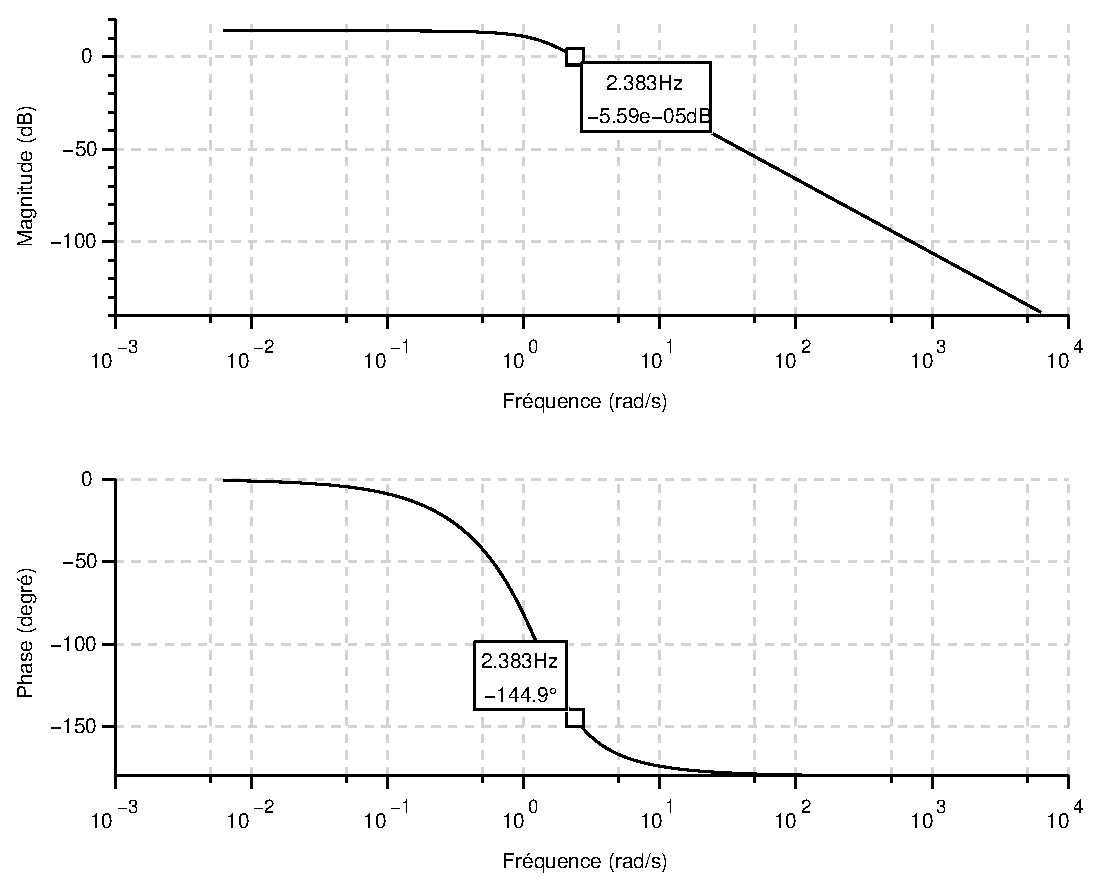
\includegraphics[width=0.75\textwidth]{bode_BONC.eps}
    \caption{Diagramme de Bode de la boucle ouverte non corrigée. 
             On a représenté le gain et la phase à la pulsation de coupure 
             $\omega_{\SI{0}{\dB}}$ du système non corrigée.}
\end{figure}
%-------------------------------------------------------------------------------
Comme attendu le déphasage est nulle à basse fréquence (BF) et de 
\SI{-180}{\degreeSI} à haute fréquence (HF) (degré 1 au numérateur et 
degré 3 au dénominateur). De même la pente du gain est nulle à BF et 
de \SI{-40}{\dB\per\dec}.
%Q2
%%%%%%%%%%%%%%%%%%%%%%%%%%%%%%%%%%%%%%%%%%%%%%%%%%%%%%%%%%%%%%%%%%%%%%%%%%%%%%%%
\question{\textbf{Déterminer la pulsation $\omega_{\SI{0}{\dB}}$, telle que le 
          gain de la fonction de transfert en boucle ouverte soit 
          égale à \SI{0}{\dB}}}
%%%%%%%%%%%%%%%%%%%%%%%%%%%%%%%%%%%%%%%%%%%%%%%%%%%%%%%%%%%%%%%%%%%%%%%%%%%%%%%%
D'après le diagramme de Bode précédent, on mesure graphiquement une pulsation
$\omega_{\SI{0}{\dB}}=\SI{2.383}{\radian\per\second}$.
Par le calcul, on déterminer cette valeur comme la pulsation qui donne un 
module de la fonction de transfert en boucle ouverte complexe égal à 1.
On cherche donc $\omega$ tel que :
%-------------------------------------------------------------------------------
\begin{align*}
    |H(j\omega)|=1 &\iff \\
    \dfrac{|10+j5\omega|}{|(2-3\omega^2)+\jw(4-\omega^2)|}=1 &\iff \\
    \dfrac{100+25\omega^2}{\omega^6+\omega^4+4\omega^2+4}=1 &\iff \\
    \omega^6+\omega^4-21\omega^2-96=0
\end{align*}
%-------------------------------------------------------------------------------
Pour résoudre cette équation, on pourrait utiliser l'instruction Scilab 
suivante :
%-------------------------------------------------------------------------------
\inputminted{scilab}{codes/scilab/code_q2_1_chap_correction.sce}
%-------------------------------------------------------------------------------
La solution réelle et positive de cette équation est bien la pulsation obtenue
graphiquement.

Il est possible de vérifier ceci en calculant le module et la phase de la 
fonction de transfert en boucle ouverte non corrigée à cette pulsation. 
(En utilisant les fonctions Scilab \texttt{repfreq} et \texttt{dbphi}). 
%-------------------------------------------------------------------------------
\inputminted{scilab}{codes/scilab/code_q2_2_chap_correction.sce}
%-------------------------------------------------------------------------------

%Q3
%%%%%%%%%%%%%%%%%%%%%%%%%%%%%%%%%%%%%%%%%%%%%%%%%%%%%%%%%%%%%%%%%%%%%%%%%%%%%%%%
\question{\textbf{Déterminer si le système est stable en boucle fermée par la 
          méthode de votre choix. Si oui, déterminer la marge de 
          phase $M_\phi$}}
%%%%%%%%%%%%%%%%%%%%%%%%%%%%%%%%%%%%%%%%%%%%%%%%%%%%%%%%%%%%%%%%%%%%%%%%%%%%%%%%
D'après le diagramme de Bode de la boucle ouverte, le système est stable 
en boucle fermée par le critère de Nyquist. On peut également le vérifier 
en déterminant les pôles de la fonction de transfert en boucle fermée.
\[
    H_{BF}=\dfrac{5p+10}{p^3+3p^2+9p+12}
\]
%-------------------------------------------------------------------------------
\inputminted{scilab}{codes/scilab/code_q3_chap_correction.sce}
%-------------------------------------------------------------------------------
Les pôles sont tous à partie réelle négative ce qui confirme la conclusion 
précédente. Le critère pourrait également être appliqué.
%Q4
%%%%%%%%%%%%%%%%%%%%%%%%%%%%%%%%%%%%%%%%%%%%%%%%%%%%%%%%%%%%%%%%%%%%%%%%%%%%%%%%
\question{\textbf{Tracer la réponse indicielle de la boucle fermée et 
          déterminer la valeur finale de la boucle fermée. On pourra donner
          certaines grandeurs caractérisant sa rapidité, son dépassement}}
%%%%%%%%%%%%%%%%%%%%%%%%%%%%%%%%%%%%%%%%%%%%%%%%%%%%%%%%%%%%%%%%%%%%%%%%%%%%%%%%
%-------------------------------------------------------------------------------
\inputminted{scilab}{codes/scilab/code_q4_chap_correction.sce}
%-------------------------------------------------------------------------------
\begin{figure}
    \centering
    \tikzsetnextfilename
    {reponse_indicielle_non_corrige-exercices_corriges-chap_correction-ext}
    \begin{tikzpicture}
    \begin{axis}
    [
        axis x line=center,
        axis y line=center,
        xlabel={$t$},
        ylabel={$s(t)$},
        x label style ={below},
        y label style ={left},
        xtick={2.5,5,7.5,10},
        xticklabels={2.5,5,7.5},
        ytick={0,0.25,0.5,0.75,1.0,1.25,1.5},
        yticklabels={0,,0.5,,1.0},
        grid=both,
        ymin=0,ymax=1.2,
    ]
    \addplot[mark=none,col4,ultra thick] 
            table {scilab/step_response_hbf_NC.dat};
    \addplot[col4,dashed,domain=0:10] {0.83333*0.95};
    \addplot[col4,dashed,domain=0:10] {0.83333*1.05};
    \end{axis}
\end{tikzpicture}

    \caption{Réponse indicielle du système en boucle fermée non corrigé}
\end{figure}
%-------------------------------------------------------------------------------
La valeur finale est graphiquement égale à 0.83 .
Par le calcul il suffit d'appliquer le théorème de la valeur finale:
\[
    \lim\limits_{p\to0} pS(p)=
    \lim\limits_{p\to0} pH_{BF}(p)E(p)=
    \lim\limits_{p\to0} H_{BF}(p)=\dfrac{5}{6}\sim0.833
\]
pour $E(p)=\dfrac{1}{p}$.
Le temps de réponse à 5\% est de l'ordre de \SI{5}{\second} et le premier 
dépassement de 40\%.
%%%%%%%%%%%%%%%%%%%%%%%%%%%%%%%%%%%%%%%%%%%%%%%%%%%%%%%%%%%%%%%%%%%%%%%%%%%%%%%%
%%%%%%%%%%%%%%%%%%%%%%%%%%%%%%%%%%%%%%%%%%%%%%%%%%%%%%%%%%%%%%%%%%%%%%%%%%%%%%%%
\subsection*{Régulation du correcteur à avance de phase}
%%%%%%%%%%%%%%%%%%%%%%%%%%%%%%%%%%%%%%%%%%%%%%%%%%%%%%%%%%%%%%%%%%%%%%%%%%%%%%%%
%%%%%%%%%%%%%%%%%%%%%%%%%%%%%%%%%%%%%%%%%%%%%%%%%%%%%%%%%%%%%%%%%%%%%%%%%%%%%%%%
On souhaite corriger le système en rapidité et en robustesse (augmenter la 
marge de stabilité). Pour augmenter la bande passante en boucle fermée, on 
décide de fixer la pulsation de coupure $\omega_0$ à 
\SI{4}{\radian\per\second} et on cherche à obtenir parallèlement une marge 
de phase $M_\phi$ de \SI{60}{\degreeSI}.

%Q5
%%%%%%%%%%%%%%%%%%%%%%%%%%%%%%%%%%%%%%%%%%%%%%%%%%%%%%%%%%%%%%%%%%%%%%%%%%%%%%%%
\question{\textbf{À partir du diagramme de Bode de la boucle ouverte 
          non corrigée, déterminer la phase $\phi_d$ et le gain $G_d$ devant 
          être apportés par le correcteur à avance de phase à la 
          pulsation de coupure que l'on s'est donnée.}}
%%%%%%%%%%%%%%%%%%%%%%%%%%%%%%%%%%%%%%%%%%%%%%%%%%%%%%%%%%%%%%%%%%%%%%%%%%%%%%%%
Le déphasage apporté par le système en boucle ouverte corrigée est donnée
par l'argument de la fonction de transfert complexe en  $\omega_0$. Soit
encore, 
\[
    \arg{\left(C_{PI}H(j\omega_0)\right)} = \phi_d + \arg{H(j\omega_0)}
\]
où $\phi_d$ est le déphasage apporté par le correcteur seul.
Pour une marge de phase souhaité de $M_\phi$. On cherche donc $\phi_d$
\[
    \phi_d=\SI{-180}{\degreeSI}+M_\phi-\arg{H(j\omega_0)}
\]
\[
    \phi_d=\SI{-120}{\degreeSI}-\arg{H(j\omega_0)}
\]
où $\arg{H(j\omega_0)}$ est le déphasage de la boucle ouverte non corrigée à 
la pulsation $\omega_0)$ (que l'on obtient graphiquement sur le diagramme de 
Bode.)
%-------------------------------------------------------------------------------
\begin{figure}
    \centering
    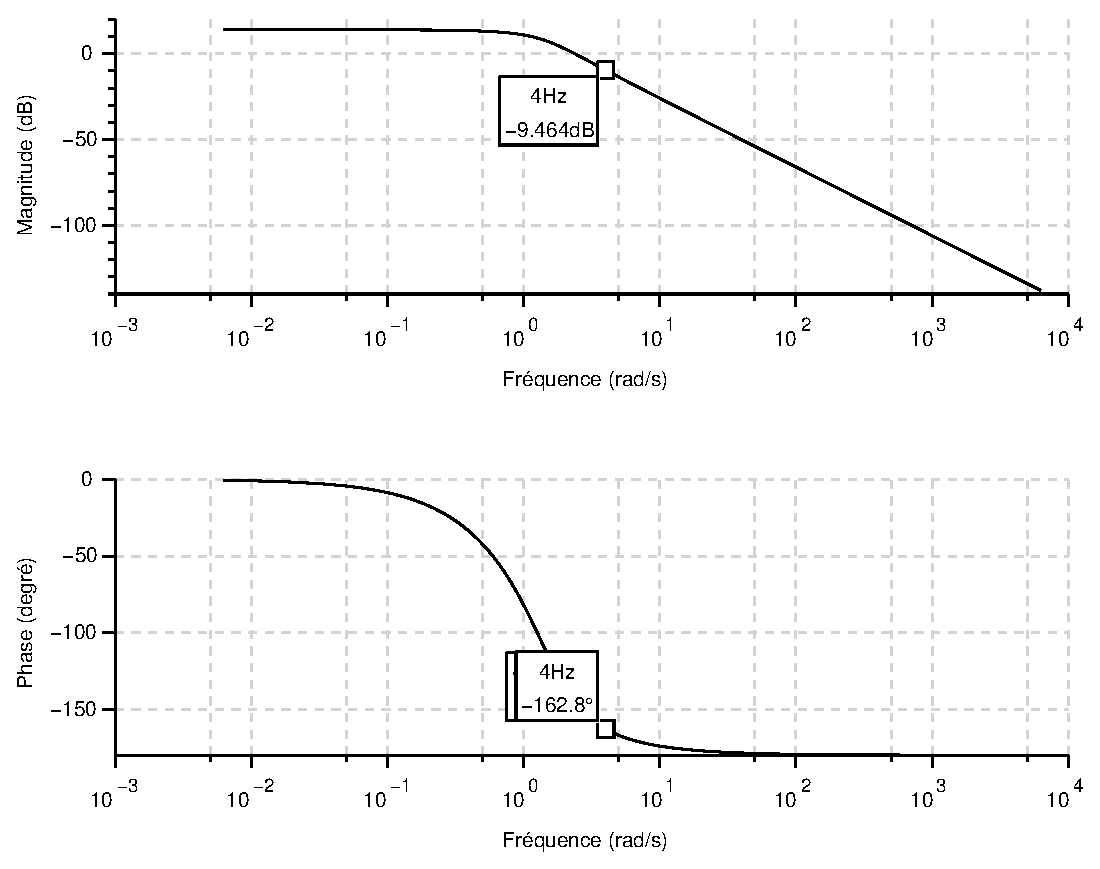
\includegraphics[width=0.75\textwidth]{bode_BONC_2.eps}
    \caption{Diagramme de Bode de la boucle ouverte non corrigée
             On a représenté le gain et la phase à la pulsation de coupure 
             $\omega_0=\SI{4}{\radian\per\second}$}
\end{figure}
%-------------------------------------------------------------------------------
On mesure $\arg{H(j\omega_0)}=\SI{-162.8}{\degreeSI}$ :
\[
    \phi_d=\SI{42.8}{\degreeSI}
\]
\[
    G_d=\SI{9.46}{\dB}=10^{9.46/20}=2.97
\]
%Q6
%%%%%%%%%%%%%%%%%%%%%%%%%%%%%%%%%%%%%%%%%%%%%%%%%%%%%%%%%%%%%%%%%%%%%%%%%%%%%%%%
\question{\textbf{À partir des relations suivantes, déterminer les paramètres 
$(\alpha,\tau_d,K_d)$ du correcteur à avance de phase}}
%%%%%%%%%%%%%%%%%%%%%%%%%%%%%%%%%%%%%%%%%%%%%%%%%%%%%%%%%%%%%%%%%%%%%%%%%%%%%%%%
On a alors :
%-------------------------------------------------------------------------------
\begin{align*}
    \alpha&=\dfrac{1+\sin\phi_d}{1-\sin\phi_d}=5.239 \\
    \tau_d&=\dfrac{1}{\omega_0\sqrt\alpha}=\SI{0.109}{\second}\\
       K_d&=\dfrac{G_d}{\sqrt\alpha}=1.298
\end{align*}
%-------------------------------------------------------------------------------
%Q7
%%%%%%%%%%%%%%%%%%%%%%%%%%%%%%%%%%%%%%%%%%%%%%%%%%%%%%%%%%%%%%%%%%%%%%%%%%%%%%%%
\question{\textbf{Donner la forme numérique de la fonction de transfert du 
          correcteur à avance de phase}}
%%%%%%%%%%%%%%%%%%%%%%%%%%%%%%%%%%%%%%%%%%%%%%%%%%%%%%%%%%%%%%%%%%%%%%%%%%%%%%%%
\[
C_{AP}(p)=\dfrac{1.298 + 0.743p } {1 + 0.109p}
\]
%Q8
%%%%%%%%%%%%%%%%%%%%%%%%%%%%%%%%%%%%%%%%%%%%%%%%%%%%%%%%%%%%%%%%%%%%%%%%%%%%%%%%
\question{\textbf{Tracer le diagramme de Bode de la boucle ouverte corrigée par 
          ce correcteur}}
%%%%%%%%%%%%%%%%%%%%%%%%%%%%%%%%%%%%%%%%%%%%%%%%%%%%%%%%%%%%%%%%%%%%%%%%%%%%%%%%
Les instructions Scilab ci-dessous permettent de tracer le diagramme 
de Bode de la boucle ouverte corrigée par un correcteur à avance de phase.
%-------------------------------------------------------------------------------
\inputminted{scilab}{codes/scilab/code_q8_chap_correction.sce}
%-------------------------------------------------------------------------------
%-------------------------------------------------------------------------------
\begin{figure}
    \centering
    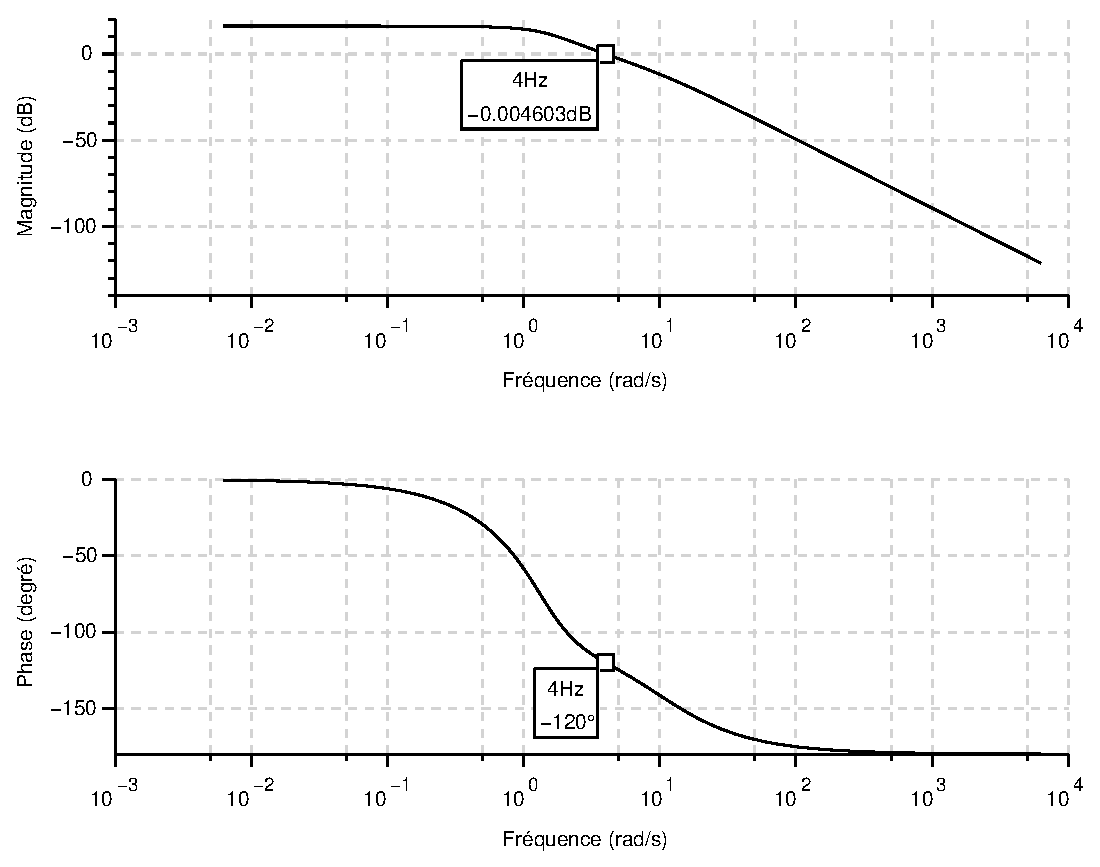
\includegraphics[width=0.75\textwidth]{bode_BOCAP.eps}
    \caption{Diagramme de Bode de la boucle ouverte corrigée par le correcteur
    à avance de phase}
\end{figure}
%-------------------------------------------------------------------------------
On vérifie bien que la marge de phase $M_\phi$ est égale à \SI{60}{\degreeSI}
à la pulsation de coupure de $\omega_0=\SI{4}{\radian\per\second}$.
%%%%%%%%%%%%%%%%%%%%%%%%%%%%%%%%%%%%%%%%%%%%%%%%%%%%%%%%%%%%%%%%%%%%%%%%%%%%%%%%
%%%%%%%%%%%%%%%%%%%%%%%%%%%%%%%%%%%%%%%%%%%%%%%%%%%%%%%%%%%%%%%%%%%%%%%%%%%%%%%%
\subsection*{Régulation du correcteur PI}
%%%%%%%%%%%%%%%%%%%%%%%%%%%%%%%%%%%%%%%%%%%%%%%%%%%%%%%%%%%%%%%%%%%%%%%%%%%%%%%%
%%%%%%%%%%%%%%%%%%%%%%%%%%%%%%%%%%%%%%%%%%%%%%%%%%%%%%%%%%%%%%%%%%%%%%%%%%%%%%%%
On souhaite maintenant rendre le système précis à l'aide de l'effet intégral
Cependant, on veut également garantir de nouveau une marge de phase $M_\phi$ de 
\SI{60}{\degree}. Pour maintenir le système stable, il faut donc centrer le 
correcteur PI à une pulsation $\omega_0<\omega_{\SI{0}{\dB}}$
%Q9
%%%%%%%%%%%%%%%%%%%%%%%%%%%%%%%%%%%%%%%%%%%%%%%%%%%%%%%%%%%%%%%%%%%%%%%%%%%%%%%%
\question{\textbf{Déterminer l'intervalle des pulsations pour laquelle 
          la marge de stabilité $M_\phi$ de \SI{60}{\degree} 
          est accessible}}
%%%%%%%%%%%%%%%%%%%%%%%%%%%%%%%%%%%%%%%%%%%%%%%%%%%%%%%%%%%%%%%%%%%%%%%%%%%%%%%%
Le déphasage apporté par le correcteur PI étant compris entre 
$\SI{-90}{\degree}$ et $\SI{0}{\degree}$, le déphasage du système 
corrigé ne peut présenter une marge de phase de $\SI{60}{\degree}$ que pour 
un certain intervalle de pulsations. En effet, puisque
\[
    \arg{H(j\omega_0)}=\SI{-180}{\degreeSI}+M_\phi-\phi_i,
\]
où $\arg{H(j\omega_0)}$ est le déphasage de la boucle ouverte non 
corrigé à la pulsation $\omega_0$ et $\phi_i$ le déphasage du 
correcteur tel que $\SI{-90}{\degreeSI}<\phi_i<\SI{0}{\degree}$. 
L'argument $\arg{H(j\omega_0)}$ est donc contraint par les 
bornes de $\phi_i$ :
\[
    \SI{-180}{\degreeSI}+M_\phi<\arg{H(j\omega_0)}<\SI{-90}{\degreeSI}+M_\phi
\]
soit pour $M_\phi=\SI{60}{\degreeSI}$
\[
    \SI{-120}{\degreeSI}<\arg{H(j\omega_0)}<\SI{-30}{\degreeSI}
\]
On peut relever sur le diagramme de Bode de la boucle ouverte non corrigée,
l'intervalle de pulsations donnant lieu à cet encadrement de la phase.
%-------------------------------------------------------------------------------
\begin{figure}
    \centering
    \includegraphics[width=0.75\textwidth]{bode_BONC_3.eps}
    \caption{Diagramme de Bode de la boucle ouverte non corrigée
             On a représenté l'intervalle de pulsations donnant 
             lieu à l'encadrement
             $\SI{-120}{\degreeSI}<\arg{H(j\omega_0)}<\SI{-30}{\degreeSI}$.}
\end{figure}
%-------------------------------------------------------------------------------
On détermine :
\[
    \SI{0.35}{\radian\per\second}<\omega_0<\SI{1.615}{\radian\per\second}
\]
La pulsation de coupure sera donc plus petite que la pulsation de coupure
du système non corrigée. On s'attend donc à un système moins rapide puisque la 
bande passante en BF devrait être également plus petite.

On choisit arbitrairement une pulsation $\omega_0=\SI{1}{\radian\per\second}$
compris dans l'intervalle précédent.
%Q10
%%%%%%%%%%%%%%%%%%%%%%%%%%%%%%%%%%%%%%%%%%%%%%%%%%%%%%%%%%%%%%%%%%%%%%%%%%%%%%%%
\question{\textbf{Déterminer le gain $G_i$ et la phase $\phi_i$ devant être
          apporté pour maintenir une marge de phase de \SI{60}{\degreeSI} 
          à cette pulsation de coupure.}}
%%%%%%%%%%%%%%%%%%%%%%%%%%%%%%%%%%%%%%%%%%%%%%%%%%%%%%%%%%%%%%%%%%%%%%%%%%%%%%%%
On peut simplement lire ces quantités sur le diagramme de Bode de la boucle
ouverte non corrigée. On obtient :
\[
    G_i=\SI{-10.97}{\dB}=10^{-10.97/20}=0.283
\]
\[
    \phi_i=\arg{H(j\omega_0)}+\SI{180}{\degreeSI}-M_\phi=\SI{38.13}{\degreeSI}
\]
avec $\arg{H(j\omega_0)}=\SI{-81.9}{\degreeSI}$ et 
$\phi_i=\arg{C_{PI}(j\omega_0)}$
%-------------------------------------------------------------------------------
\begin{figure}
    \centering
    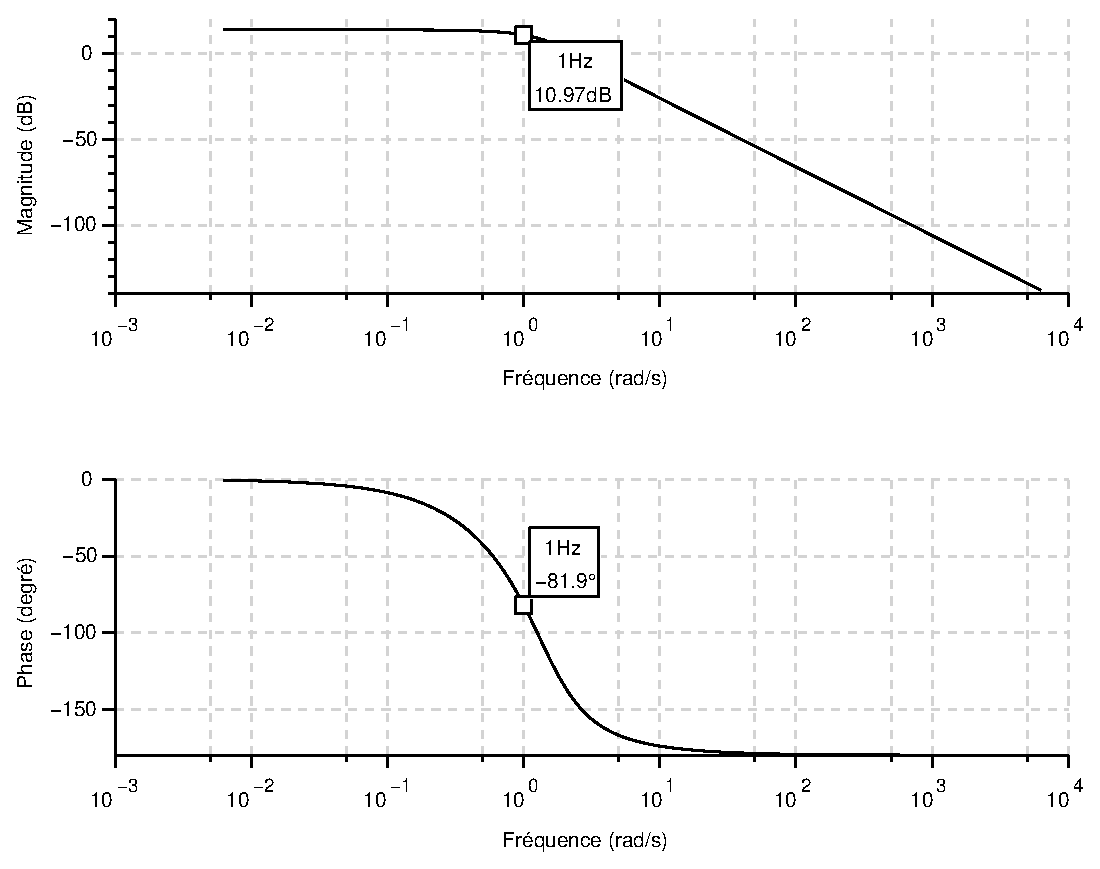
\includegraphics[width=0.75\textwidth]{bode_BONC_4.eps}
    \caption{Diagramme de Bode de la boucle ouverte non corrigée
             On a représenté le gain et la phase à la pulsation de coupure 
             $\omega_0=\SI{1}{\radian\per\second}$}
\end{figure}
%-------------------------------------------------------------------------------
%Q11
%%%%%%%%%%%%%%%%%%%%%%%%%%%%%%%%%%%%%%%%%%%%%%%%%%%%%%%%%%%%%%%%%%%%%%%%%%%%%%%%
\question{\textbf{Déterminer les paramètres $\tau_i$ et $K_i$ à partir des 
          relations du correcteur PI suivantes:}}
%%%%%%%%%%%%%%%%%%%%%%%%%%%%%%%%%%%%%%%%%%%%%%%%%%%%%%%%%%%%%%%%%%%%%%%%%%%%%%%%
%-------------------------------------------------------------------------------
\begin{align*}
    \tau_i=-\dfrac{1}{\omega_0\tan\phi_i}=\SI{1.27}{\second}\\
    K_i=\dfrac{G_i\tau_i\omega_0}{\sqrt{1+\tau^2_i\omega^2_0}}=0.222
\end{align*}
%-------------------------------------------------------------------------------
%Q12
%%%%%%%%%%%%%%%%%%%%%%%%%%%%%%%%%%%%%%%%%%%%%%%%%%%%%%%%%%%%%%%%%%%%%%%%%%%%%%%%
\question{\textbf{Donner la forme numérique de la fonction de transfert du 
          régulateur PI ainsi obtenu}}
%%%%%%%%%%%%%%%%%%%%%%%%%%%%%%%%%%%%%%%%%%%%%%%%%%%%%%%%%%%%%%%%%%%%%%%%%%%%%%%%
\[
    C_{PI}(p)=\dfrac{0.222 + 0.283p}{1.274p}
\]
%Q13
%%%%%%%%%%%%%%%%%%%%%%%%%%%%%%%%%%%%%%%%%%%%%%%%%%%%%%%%%%%%%%%%%%%%%%%%%%%%%%%%
\question{\textbf{Tracer le diagramme de Bode de la boucle ouverte corrigée 
          par ce correcteur}}
%%%%%%%%%%%%%%%%%%%%%%%%%%%%%%%%%%%%%%%%%%%%%%%%%%%%%%%%%%%%%%%%%%%%%%%%%%%%%%%%
%-------------------------------------------------------------------------------
\inputminted{scilab}{codes/scilab/code_q13_chap_correction.sce}
%-------------------------------------------------------------------------------
%-------------------------------------------------------------------------------
\begin{figure}
    \centering
    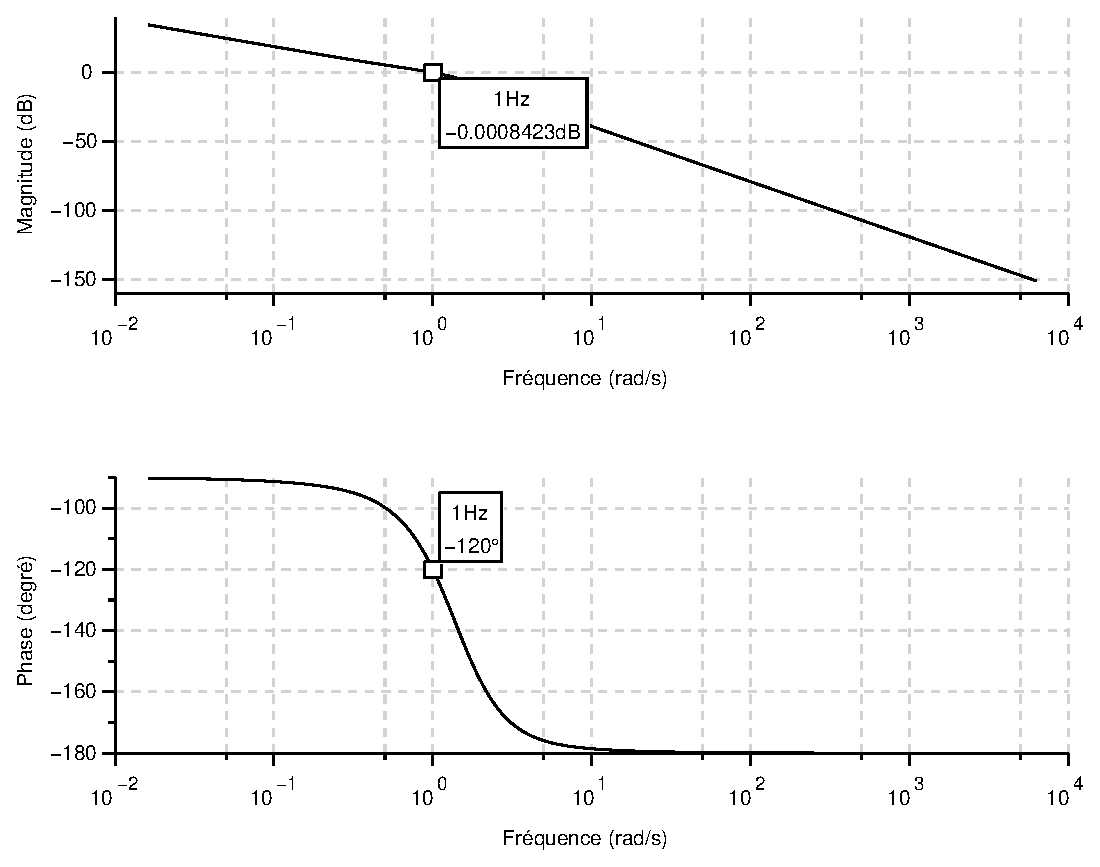
\includegraphics[width=0.75\textwidth]{bode_BOCPI.eps}
    \caption{Diagramme de Bode de la boucle ouverte corrigée par 
    le correcteur PI}
\end{figure}
%-------------------------------------------------------------------------------
On vérifie qu'à la pulsation de coupure le gain est nul (en \si{\dB}) et
que la phase donne une marge de phase de \SI{60}{\degreeSI}
%%%%%%%%%%%%%%%%%%%%%%%%%%%%%%%%%%%%%%%%%%%%%%%%%%%%%%%%%%%%%%%%%%%%%%%%%%%%%%%%
%%%%%%%%%%%%%%%%%%%%%%%%%%%%%%%%%%%%%%%%%%%%%%%%%%%%%%%%%%%%%%%%%%%%%%%%%%%%%%%%
\subsection*{Régulation du correcteur PID}
%%%%%%%%%%%%%%%%%%%%%%%%%%%%%%%%%%%%%%%%%%%%%%%%%%%%%%%%%%%%%%%%%%%%%%%%%%%%%%%%
%%%%%%%%%%%%%%%%%%%%%%%%%%%%%%%%%%%%%%%%%%%%%%%%%%%%%%%%%%%%%%%%%%%%%%%%%%%%%%%%
%Q14
%%%%%%%%%%%%%%%%%%%%%%%%%%%%%%%%%%%%%%%%%%%%%%%%%%%%%%%%%%%%%%%%%%%%%%%%%%%%%%%%
\question{\textbf{En utilisant la méthodologie précédente, déterminer les 
          paramètres des régulateurs composant ce PID}}
%%%%%%%%%%%%%%%%%%%%%%%%%%%%%%%%%%%%%%%%%%%%%%%%%%%%%%%%%%%%%%%%%%%%%%%%%%%%%%%%
La résolution du système de deux équations suivant:
\[
\begin{cases}
    \phi_d-\phi_i&=\SI{-180}{\degreeSI}+M_\phi-\arg{H(j\omega_0)} \\
    \phi_d+\phi_i&=\SI{90}{\degreeSI},
\end{cases}
\]
nous permet de déterminer numériquement les phases $\phi_d$ et 
$\phi_i$ des correcteurs. On obtient alors:
\[
\begin{cases}
    \phi_d=\SI{-45}{\degreeSI}+
           \dfrac{M_\phi-\arg{H(j\omega_0)}}{2}=\SI{66.39}{\degreeSI} \\
    \phi_i=\SI{135}{\degreeSI}+
           \dfrac{\arg{H(j\omega_0)}-M_\phi}{2}=\SI{23.61}{\degreeSI}
\end{cases}
\]

On a alors pour les paramètres des correcteurs :
%-------------------------------------------------------------------------------
\begin{itemize}
    \item[AP] 
%-------------------------------------------------------------------------------
        \begin{align*}
            \alpha&=22.89\\
            \tau_d&=\SI{0.052}{\second}\\
            K_d&=0.209
        \end{align*}
%-------------------------------------------------------------------------------
    \item[PI]
%-------------------------------------------------------------------------------
        \begin{align*}
            \tau_i&=\SI{0.572}{\second}\\
            k_i&=0.9163
        \end{align*}
%-------------------------------------------------------------------------------

\[
    k_p=2.97
\]
\end{itemize}
%-------------------------------------------------------------------------------
%Q15
%%%%%%%%%%%%%%%%%%%%%%%%%%%%%%%%%%%%%%%%%%%%%%%%%%%%%%%%%%%%%%%%%%%%%%%%%%%%%%%%
\question{\textbf{Donner la forme numérique de la fonction de transfert du 
          correcteur}}
%%%%%%%%%%%%%%%%%%%%%%%%%%%%%%%%%%%%%%%%%%%%%%%%%%%%%%%%%%%%%%%%%%%%%%%%%%%%%%%%
\[
    C_{AP}(p)=\dfrac{0.208 + 0.25p}{1+0.052p}
\]
\[
    C_{PI}(p)=\dfrac{0.916 + 0.524p}{0.572p}
\]
\[
    C_{PID}(p)=\dfrac{0.569+1.006p+0.389p^2}{0.572p+ 0.029p^2}  
\]
%Q16
%%%%%%%%%%%%%%%%%%%%%%%%%%%%%%%%%%%%%%%%%%%%%%%%%%%%%%%%%%%%%%%%%%%%%%%%%%%%%%%%
\question{\textbf{Tracer le diagramme de Bode de la boucle ouverte corrigée}}
%%%%%%%%%%%%%%%%%%%%%%%%%%%%%%%%%%%%%%%%%%%%%%%%%%%%%%%%%%%%%%%%%%%%%%%%%%%%%%%%
%-------------------------------------------------------------------------------
\inputminted{scilab}{codes/scilab/code_q16_chap_correction.sce}
%-------------------------------------------------------------------------------
%-------------------------------------------------------------------------------
\begin{figure}
    \centering
    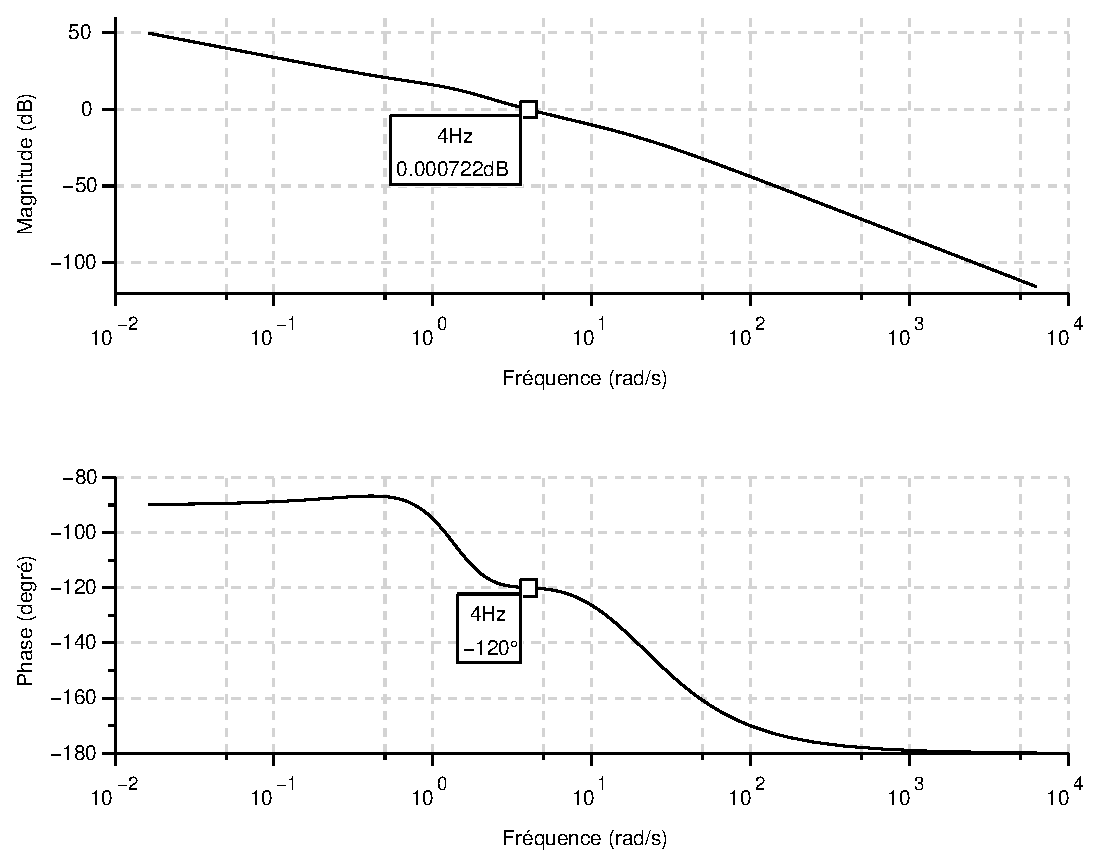
\includegraphics[width=0.75\textwidth]{bode_BOCPID.eps}
    \caption{Diagramme de Bode de la boucle ouverte corrigée par 
    le correcteur PID}
\end{figure}
%-------------------------------------------------------------------------------
On vérifie la phase et le gain à la pulsation de coupure.
%%%%%%%%%%%%%%%%%%%%%%%%%%%%%%%%%%%%%%%%%%%%%%%%%%%%%%%%%%%%%%%%%%%%%%%%%%%%%%%%
%%%%%%%%%%%%%%%%%%%%%%%%%%%%%%%%%%%%%%%%%%%%%%%%%%%%%%%%%%%%%%%%%%%%%%%%%%%%%%%%
\subsection*{Réponses temporelles en boucle fermée}
%%%%%%%%%%%%%%%%%%%%%%%%%%%%%%%%%%%%%%%%%%%%%%%%%%%%%%%%%%%%%%%%%%%%%%%%%%%%%%%%
%%%%%%%%%%%%%%%%%%%%%%%%%%%%%%%%%%%%%%%%%%%%%%%%%%%%%%%%%%%%%%%%%%%%%%%%%%%%%%%%
%Q17
%%%%%%%%%%%%%%%%%%%%%%%%%%%%%%%%%%%%%%%%%%%%%%%%%%%%%%%%%%%%%%%%%%%%%%%%%%%%%%%%
\question{\textbf{Comparer sur une figure les diagrammes de Bode de ces boucles 
          ouvertes corrigées et non corrigées}}
%%%%%%%%%%%%%%%%%%%%%%%%%%%%%%%%%%%%%%%%%%%%%%%%%%%%%%%%%%%%%%%%%%%%%%%%%%%%%%%%

%-------------------------------------------------------------------------------
\begin{figure}[!h]
    \centering
    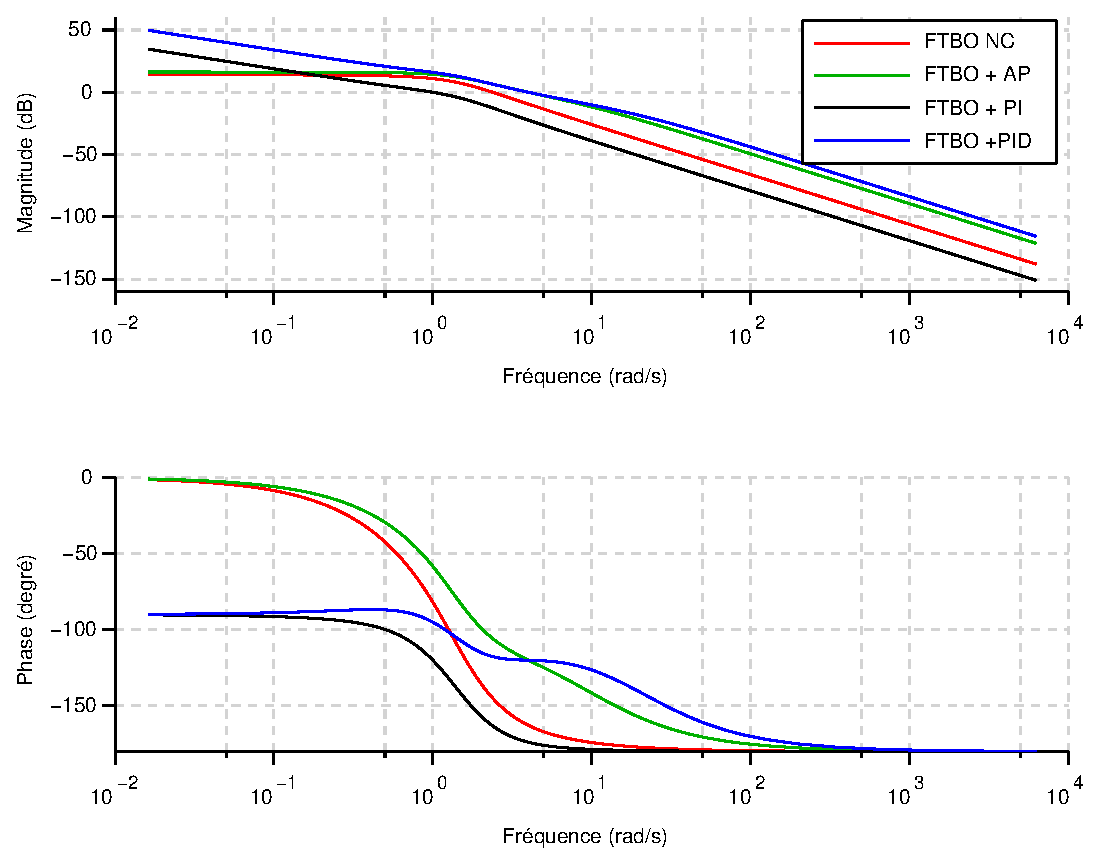
\includegraphics[width=0.75\textwidth]{bode_BOC_all.eps}
    \caption{Diagramme de Bode de la boucle ouverte corrigée par 
    le correcteur PID}
\end{figure}
%-------------------------------------------------------------------------------
\clearpage
%Q18
%%%%%%%%%%%%%%%%%%%%%%%%%%%%%%%%%%%%%%%%%%%%%%%%%%%%%%%%%%%%%%%%%%%%%%%%%%%%%%%%
\question{\textbf{Tracer les réponses indicielles en boucle fermée de tous ces 
          correcteurs. Conclure ses les performances corrigées.}}
%%%%%%%%%%%%%%%%%%%%%%%%%%%%%%%%%%%%%%%%%%%%%%%%%%%%%%%%%%%%%%%%%%%%%%%%%%%%%%%%
%-------------------------------------------------------------------------------
\begin{figure}
\centering
\tikzsetnextfilename
{reponse_indicielle_corrigee-exercices_corriges-chap_correction-ext}
\input{tikz/reponse_indicielle_corrigee-exercices_corriges-chap_correction.tex}
\caption{Réponse indicielle du système en boucle fermée non corrigé 
         et corrigé par les différents régulateurs 
         du TD.~\label{fig-reponses_indicielles}}
\end{figure}
%-------------------------------------------------------------------------------
On a tracé sur la même figure~\ref{fig-reponses_indicielles} en boucle fermée 
de tout les systèmes corrigés et non corrigés du TD. On observe clairement les
effets de chacun d'entre eux:
%-------------------------------------------------------------------------------
\begin{itemize}
%-------------------------------------------------------------------------------
    \item Avance de phase: 
%-------------------------------------------------------------------------------
        \begin{itemize}
            \item augmentation de la marge de stabilité 
                  (moins d'oscillations, réduction du déplacement)
            \item augmentation de la bande passante et donc de la rapidité
            \item le système n'est pas précis (elle augmente cependant par 
                  rapport au système non corrigé)
        \end{itemize}
%-------------------------------------------------------------------------------
    \item Proportionnel Intégral : 
%-------------------------------------------------------------------------------
        \begin{itemize}
            \item effet intégral : système précis et diminution de la rapidité 
        \end{itemize} 
%-------------------------------------------------------------------------------
    \item Proportionnel Intégral Dérivé :
%-------------------------------------------------------------------------------
        \begin{itemize}
            \item effet intégral : système précis
            \item effet dérivé : augmentation de la rapidité et 
                  diminution des oscillations.
        \end{itemize} 
%-------------------------------------------------------------------------------
\end{itemize}
%-------------------------------------------------------------------------------
\clearpage
%%%%%%%%%%%%%%%%%%%%%%%%%%%%%%%%%%%%%%%%%%%%%%%%%%%%%%%%%%%%%%%%%%%%%%%%%%%%%%%%
%%%%%%%%%%%%%%%%%%%%%%%%%%%%%%%%%%%%%%%%%%%%%%%%%%%%%%%%%%%%%%%%%%%%%%%%%%%%%%%%
\subsection*{Code Scilab complet}
%%%%%%%%%%%%%%%%%%%%%%%%%%%%%%%%%%%%%%%%%%%%%%%%%%%%%%%%%%%%%%%%%%%%%%%%%%%%%%%%
%%%%%%%%%%%%%%%%%%%%%%%%%%%%%%%%%%%%%%%%%%%%%%%%%%%%%%%%%%%%%%%%%%%%%%%%%%%%%%%%
%-------------------------------------------------------------------------------
\inputminted{scilab}{codes/scilab/code_exercice_chap_correction.sce}
%-------------------------------------------------------------------------------

\normalsize
\restoregeometry
\captionsetup{width=0.9\linewidth}
%%%%%%%%%%%%%%%%%%%%%%%%%%%%%%%%%%%%%%%%%%%%%%%%%%%%%%%%%%%%%%%%%%%%%%%%%%%%%%%%
%%%%%%%%%%%%%%%%%%%%%%%%%%%%%%%%%%%%%%%%%%%%%%%%%%%%%%%%%%%%%%%%%%%%%%%%%%%%%%%%
%%%%%%%%%%%%%%%%%%%%%%%%%%%%%%%%%%%%%%%%%%%%%%%%%%%%%%%%%%%%%%%%%%%%%%%%%%%%%%%%
%%%%%%%%%%%%%%%%%%%%%%%%%%%%%%%%%%%%%%%%%%%%%%%%%%%%%%%%%%%%%%%%%%%%%%%%%%%%%%%%
%chap_correction.tex
